\chapter{Subsequent Motion Correction: Using Advanced Reconstruction and Gating Methods with More Challenging Data} \label{sec:subsequent_motion_correction_using_advanced_reconstruction_and_gating_methods_with_more_challenging_data}
    \vspace*{\fill}
    \setlength{\epigraphwidth}{0.3\linewidth}
    \renewcommand{\epigraphflush}{flushright}
    \renewcommand{\epigraphsize}{\footnotesize}
    \epigraph{Breathe, breathe in the air}%
              {\textit{Breathe (In the Air)}\\ \textsc{Pink Floyd}}
    
    \newpage
    
    \section{Introduction} \label{sec:subsequent_motion_correction_using_advanced_reconstruction_and_gating_methods_with_more_challenging_data_introduction}
        This chapter of the thesis contains part of the work performed in the domain of motion correction. Specifically this section highlights the subsequent work on motion correction which mainly used more complex simulation data and focused on \gls{MLACF} reconstruction.
        
        The first section of this chapter introduces work to investigate the impact of using \glspl{MM} to allow for motion correction to be performed on coarsely gated data and then applied to finely gated data.
        
        The second section of this chapter highlights an evaluation of the impact of \gls{2D} and \gls{1D} gating as well as showing the impact of using \gls{MLACF} or \gls{OSEM} for reconstruction prior to motion correction.
        
        Finally, the third section of this chapter discusses the problems or limitations of the work performed in the previous two sections with reference to where problems and limitations highlighted in~\Fref{sec:initial_motion_correction_using_basic_reconstruction_and_gating_methods_with_less_challenging_data_discussion} have been addressed.
    
    \section{PET/CT Motion Correction Exploiting Motion Models Fit on Coarsely Gated Data Applied to Finely Gated Data} \label{sec:pet_ct_motion_correction_exploiting_motion_models_fit_on_coarsely_gated_data_applied_to_finely_gated_data}
        This section investigates the impact of gating coarseness on motion correction performance, with respect to the noise present in each gate. Furthermore, this section introduces a motion correction method which uses \gls{MLACF} reconstructions as part of the \gls{MM} fitting. \gls{MLACF} is used in contrast to previous work where \gls{OSEM} was used for the same purpose, as seen in~\Fref{sec:initial_motion_correction_using_basic_reconstruction_and_gating_methods_with_less_challenging_data}.

        \subsection{Introduction} \label{sec:pet_ct_motion_correction_exploiting_motion_models_fit_on_coarsely_gated_data_applied_to_finely_gated_data_introduction}
            Motion correction is imperative to the reduction of blurring and artefacts inherent in \gls{PET}. This is due to the relatively long acquisition time, and the temporal difference in the \gls{Mu-Map} acquisition. Registration literature contains many examples of spatial regularisers, however there are few temporal regularisers. \glspl{MM} can act as such a temporal regulariser, as well as allowing for the interpolation of unseen motion correction results. In previous work, a motion modelling approach to high \gls{TOF} resolution \gls{NAC} data was applied, where the data was corrected to the space of the \gls{Mu-Map}. However, this approach was challenging, especially when low contrast lung tumours are present. This work seeks to extend previous work, by incorporating an approach suggested by~\parencite{Lu2018RespiratoryData}, to perform an initial \gls{MLACF} reconstruction for the motion estimation. In this work, these two approaches are combined, with several improvements. \gls{Mu-Map} alignment, as well as, fitting the \gls{MM} on low noise low temporal/gate resolution data, and applying it to high noise high temporal/gate resolution data.% To test this, \gls{XCAT} volumes are constructed, and \gls{TOF} data simulated. Evaluation compares the results of the proposed method against, where the \gls{MM} was fit on data gated more finely, where the \gls{MM} was fit on noiseless data, and finally non-motion corrected examples. Results indicate that the incorporation of \gls{MLACF}, and fitting of the \gls{MM} on low noise low temporal/gate resolution data, improves contrast and quantification, while allowing for a relatively fast execution time.
            
            Motion Models parameterise \glspl{DVF} in terms of a \gls{SS}. They could be considered as an addition to a standard spatially regularised motion correction technique, as they impose a degree of temporal or gate-wise regularisation. In addition, they also allow obtaining \glspl{DVF} for time points/gates, not used to fit the model (as long as a relevant \gls{SS} exists~\parencite{McClelland2013}). \glspl{MM} have seen attention, particularly in \gls{CT}~\parencite{Li2007EnhancedModel}, but also \gls{MR}~\parencite{Manke2002RespiratoryModels, Manber2016JointCorrection}, however less so in clinical \gls{PET}/\gls{CT}.
            
            In previous work~\parencite{Whitehead2019ImpactPET, Whitehead2020PET/CTFields, Whitehead2021ComparisonMap}, the possibility of incorporating \glspl{MM}, in a motion correction framework, for \gls{NAC} \gls{TOF} \gls{PET}, where the reference was set to the position of a breath hold \gls{Mu-Map}, was investigated. This method could be used to deform both the gates to the reference position as well as the reference position to the gates. Preliminary experiments indicated that the combination of both the \gls{MM} and \gls{TOF}, allowed for an \gls{AC} reconstruction with motion correction, without introducing artefacts, while increasing resolution and quantification accuracy (for simulations with high \gls{TOF} resolution and count levels). This work seeks to extend the method further, using more realistic simulation and count levels, from existing clinical scanners. Firstly, by incorporating \gls{MLACF} as an initialisation technique, which provides volumes with greater contrast than \gls{NAC}, without introducing bias due to misalignment with a fixed \gls{Mu-Map}~\parencite{Nuyts2012ML-reconstructionFactors}. Secondly, low noise low temporal/gate resolution data is used to fit the \gls{MM}, while high noise high temporal/gate resolution data is used for the output. This potentially allows for reduced mis-registration, as well as improving computation time. Thirdly, a diffeomorphic velocity field parameterised registration was used, which provided \glspl{DVF} free from folding.
            
            A method incorporating \glspl{MM} for dynamic \gls{PET}/\gls{CT}, was proposed in~\parencite{Chan2018Non-RigidPET}. Additionally, a method incorporating \gls{MLACF} for \gls{PET}/\gls{CT}, was presented in~\parencite{Lu2018RespiratoryData}. The work displayed here, differentiates itself, not only by the ways mentioned above, but also by using a \gls{2D} \gls{SS} (rather than a \gls{1D} \gls{SS}). Thus, allowing more general parametrisation of the motion (here in terms of both displacement and velocity). Additionally, the group-wise method, presented here, makes use of an iterative motion correction algorithm, rather than relying only on a pair-wise method.
        
        \subsection{Methods} \label{sec:pet_ct_motion_correction_exploiting_motion_models_fit_on_coarsely_gated_data_applied_to_finely_gated_data_methods}
            \gls{AC} volumes are reconstructed using \gls{MLACF} (both `phase' gated into four and amplitude gated into $30$ bins), as seen in~\Fref{sec:pet_ct_motion_correction_exploiting_motion_models_fit_on_coarsely_gated_data_applied_to_finely_gated_data_methods_xcat_volume_generation}, ~\Fref{sec:pet_ct_motion_correction_exploiting_motion_models_fit_on_coarsely_gated_data_applied_to_finely_gated_data_methods_pet_acquisition_simulation}, and~\Fref{sec:pet_ct_motion_correction_exploiting_motion_models_fit_on_coarsely_gated_data_applied_to_finely_gated_data_methods_mlacf_image_reconstruction}. These volumes are used as input for group-wise registration and \gls{MM} estimation, as seen in~\Fref{sec:pet_ct_motion_correction_exploiting_motion_models_fit_on_coarsely_gated_data_applied_to_finely_gated_data_methods_registration} and~\Fref{sec:pet_ct_motion_correction_exploiting_motion_models_fit_on_coarsely_gated_data_applied_to_finely_gated_data_methods_motion_model_estimation}. The reference \gls{PET} volume, from the previous step, is then registered to a single \gls{Mu-Map}, at end inhalation. The resultant \gls{MM} and its inverse are used to perform a motion compensated \gls{AC} reconstruction, as seen in~\Fref{sec:pet_ct_motion_correction_exploiting_motion_models_fit_on_coarsely_gated_data_applied_to_finely_gated_data_methods_mc_image_reconstruction_with_ac}.
            
            For validation, \gls{XCAT} simulations are used, for one bed position, with a \gls{FOV} including the base of the lungs and the diaphragm. The output for data `phase' gated into four and amplitude gated into $30$ bins is evaluated against the following. Firstly, the above procedure was additionally performed (for both data `phase' gated into four and amplitude gated into $30$ bins) where the registration and \gls{MM} fitting was performed on noiseless data. Secondly, a non-motion corrected reconstruction of the same data (using a single static \gls{Mu-Map} and a \gls{Mu-Map} averages from \gls{CCT} for attenuation correction). Evaluations performed included a visual analysis (\gls{SSIM}), an examination of profile, and \gls{SUV} analysis, seen in~\Fref{sec:pet_ct_motion_correction_exploiting_motion_models_fit_on_coarsely_gated_data_applied_to_finely_gated_data_methods_evaluation}.
            
            \subsubsection{XCAT Volume Generation} \label{sec:pet_ct_motion_correction_exploiting_motion_models_fit_on_coarsely_gated_data_applied_to_finely_gated_data_methods_xcat_volume_generation}
                \gls{XCAT}~\parencite{Segars2010} was used to generate $480$ volumes over a \SI{240}{\second} period, using respiratory traces, derived from \gls{2D} \gls{CMR} patient data. The maximum displacement of \gls{AP} and \gls{SI} motion, was set to \SI{1.2}{\centi\metre} and \SI{2.0}{\centi\metre} respectively. Activity concentrations were derived from a static \gls{18F-FDG} patient scan. The \gls{FOV} included the base of the lungs, diaphragm, and the top of the liver. A \SI{20}{\milli\metre} diameter spherical lesion (smaller than the max displacement due to respiratory motion) was placed into the base of the right lung (within the maximum displacement due to respiratory motion of the diaphragm).
            
            \subsubsection{PET Acquisition Simulation} \label{sec:pet_ct_motion_correction_exploiting_motion_models_fit_on_coarsely_gated_data_applied_to_finely_gated_data_methods_pet_acquisition_simulation}
                \gls{PET} acquisitions were simulated (and reconstructed), using \gls{STIR}~\parencite{Thielemans2012, Nikos2019} through \gls{SIRF}~\parencite{Ovtchinnikov2017}, to forward project data using the geometry of a \gls{GE} Discovery $710$. Attenuation was included using the relevant \glspl{Mu-Map} generated by \gls{XCAT}. Pseudo-randoms and scatter were added. Randoms were added by summing a scaled uniform forward projection to the simulation sinogram. Pseudo-scatter was added by summing a scaled and smoothed forward projection of the activity data at each time point to the simulation sinogram. The smoothing parameter was optimised to give scatter with a similar distribution to a GATE simulation. A full scatter simulation was not performed due to software limitations.
                
                Noise was simulated, such that data matched an acquisition over \SI{240}{\second}, emulating a standard single bed position acquisition. The count rate was selected to match that of research scans, below that of diagnostic clinical scans. This count rate was selected as a `worst case scenario'.
                
                A respiratory \gls{SS} was generated using \gls{PCA}~\parencite{Thielemans2011}. The value of this signal, and its gradient, was used for gating. For \gls{MM} estimation, data were initially pseudo-phase gated. The data was displacement and gradient gated into four bins, where each bin was a quadrant centred on the maximum or minimum of the displacement or gradient. This is useful as it gives a small number of gates while allowing to fit a \gls{2D} \gls{MM} (a plane). For the purpose of the \gls{MM} fitting, \gls{SS} values were determined for the post-gated data by taking an average of the \gls{SS} values in each bin.
                
            \subsubsection{MLACF Image Reconstruction} \label{sec:pet_ct_motion_correction_exploiting_motion_models_fit_on_coarsely_gated_data_applied_to_finely_gated_data_methods_mlacf_image_reconstruction}
                Data were reconstructed using \gls{MLACF}, with seven full iterations and $24$ subsets for the activity update, and nine iterations for the attenuation update~\parencite{Nuyts2012ML-reconstructionFactors}. \gls{MLACF} was initialised using one iteration of \gls{MLEM}, where the breath hold \gls{CT} was used for attenuation correction (the \gls{ACF} were still initialised with all ones), this gave a small improvement to results without introducing bias. Between iterations, the activity volume and \gls{ACF} sinogram were normalised (scaled to the same magnitude as an equivalent volume/sinogram filled with ones), and a small value was added to each voxel, this was to aid with stabilising the reconstruction. A quadratic prior was included in the reconstruction, to promote smoothness of the \gls{ACF} sinogram.
            
            \subsubsection{Registration} \label{sec:pet_ct_motion_correction_exploiting_motion_models_fit_on_coarsely_gated_data_applied_to_finely_gated_data_methods_registration}
                Before being registered, each volume underwent pre-processing, including replication of end-slices, smoothing, and standardisation. This pre-processing was only applied to intermediate data, and was not used for the final output of the method.
                
                Group-wise registration was used, where after an initial pair-wise registration step, a new reference volume was resampled. Registration to the new reference volume, followed by another resample, continued for a set number of iterations. NiftyReg~\parencite{Modat2010} was used to perform registrations, using a diffeomorphic velocity field B-spline parameterisation. \gls{CPG} spacing of the B-spline coefficients, bending energy regularisation term weight, and number of iterations were tuned using a grid search.
                
                Between each iteration, the resampled volume was registered to the position of the \gls{Mu-Map}. The \glspl{DVF} for both the group-wise registration, and \gls{Mu-Map} registration were composed together to form one final \gls{DVF}. With the diffeomorphic nature of the registration, this would give a \gls{MM} which could generate \glspl{DVF} to and from the gates to the \gls{Mu-Map}.
            
            \subsubsection{Motion Model Estimation} \label{sec:pet_ct_motion_correction_exploiting_motion_models_fit_on_coarsely_gated_data_applied_to_finely_gated_data_methods_motion_model_estimation}
                \glspl{MM} were fit as a direct \gls{RCM} on the \glspl{CPG}, from~\Fref{sec:pet_ct_motion_correction_exploiting_motion_models_fit_on_coarsely_gated_data_applied_to_finely_gated_data_methods_registration} and the \gls{SS} from~\Fref{sec:pet_ct_motion_correction_exploiting_motion_models_fit_on_coarsely_gated_data_applied_to_finely_gated_data_methods_pet_acquisition_simulation}. A weighted linear regression was used, where the weighting was taken based on the number of counts in each gate. Once a \gls{MM} was fit, new \glspl{DVF} were generated for each gate, using the \gls{SS} values that were used to fit the \gls{MM}. \gls{MM} fitting occurred between iterations, the \glspl{DVF} generated by the \gls{MM} were used to resample the new target volume at each iteration.
            
            \subsubsection{Motion Corrected Image Reconstruction with Attenuation Correction} \label{sec:pet_ct_motion_correction_exploiting_motion_models_fit_on_coarsely_gated_data_applied_to_finely_gated_data_methods_mc_image_reconstruction_with_ac}
                Data were re-gated, using the value of \gls{SS}, and its gradient, to gate data into $30$ respiratory bins ($10$ displacement and three gradient bins).
                
                Data were re-reconstructed with attenuation correction, deforming the \glspl{Mu-Map}, using the inverse of the \glspl{DVF} determined taking the \gls{MM} from~\Fref{sec:pet_ct_motion_correction_exploiting_motion_models_fit_on_coarsely_gated_data_applied_to_finely_gated_data_methods_motion_model_estimation}. For reconstruction, \gls{OSEM} was utilised, with two full iterations and $24$ subsets (as in clinical practice)~\parencite{Hudson1994}. Motion correction was then applied, using \glspl{DVF} determined taking the \gls{MM} from~\Fref{sec:pet_ct_motion_correction_exploiting_motion_models_fit_on_coarsely_gated_data_applied_to_finely_gated_data_methods_motion_model_estimation}. Volumes were post-filtered employing a Gaussian smoothing, with a \gls{FWHM} of \SI{6.4}{\milli\metre} in the transverse plane, and a normal Z-filter (as in clinical practice).
            
            \subsubsection{Evaluation} \label{sec:pet_ct_motion_correction_exploiting_motion_models_fit_on_coarsely_gated_data_applied_to_finely_gated_data_methods_evaluation}
                In addition to the reconstructions performed in~\Fref{sec:pet_ct_motion_correction_exploiting_motion_models_fit_on_coarsely_gated_data_applied_to_finely_gated_data_methods_mc_image_reconstruction_with_ac}, motion correction was also applied to data in the same way, as in~\Fref{sec:pet_ct_motion_correction_exploiting_motion_models_fit_on_coarsely_gated_data_applied_to_finely_gated_data_methods_registration} and~\Fref{sec:pet_ct_motion_correction_exploiting_motion_models_fit_on_coarsely_gated_data_applied_to_finely_gated_data_methods_motion_model_estimation} but using high noise, high temporal/gate resolution, or noiseless data, for the \gls{MM} fitting. Furthermore, data were also reconstructed without motion correction, using either the end inhalation \gls{Mu-Map}, or a sum of all \glspl{Mu-Map} (to emulate an \gls{AV-CCT}). For the present evaluation, the volumes without motion correction were registered to the position of the end inhalation \gls{Mu-Map}. Additionally, \glspl{DVF} generated by each method were also applied to the original \gls{XCAT} volumes, for visual analysis.
                
                Comparisons made included a visual analysis, \gls{SSIM} to the ground truth~\parencite{Wang2009MeanMeasures}, a profile over the lesion, and \gls{SUV}\textsubscript{max} and \gls{SUV}\textsubscript{peak} (defined following \gls{EANM} guidelines~\parencite{Boellaard2015FDG2.0}).
        
        \subsection{Results} \label{sec:pet_ct_motion_correction_exploiting_motion_models_fit_on_coarsely_gated_data_applied_to_finely_gated_data_results}
            \begin{figure}
                \centering
                
                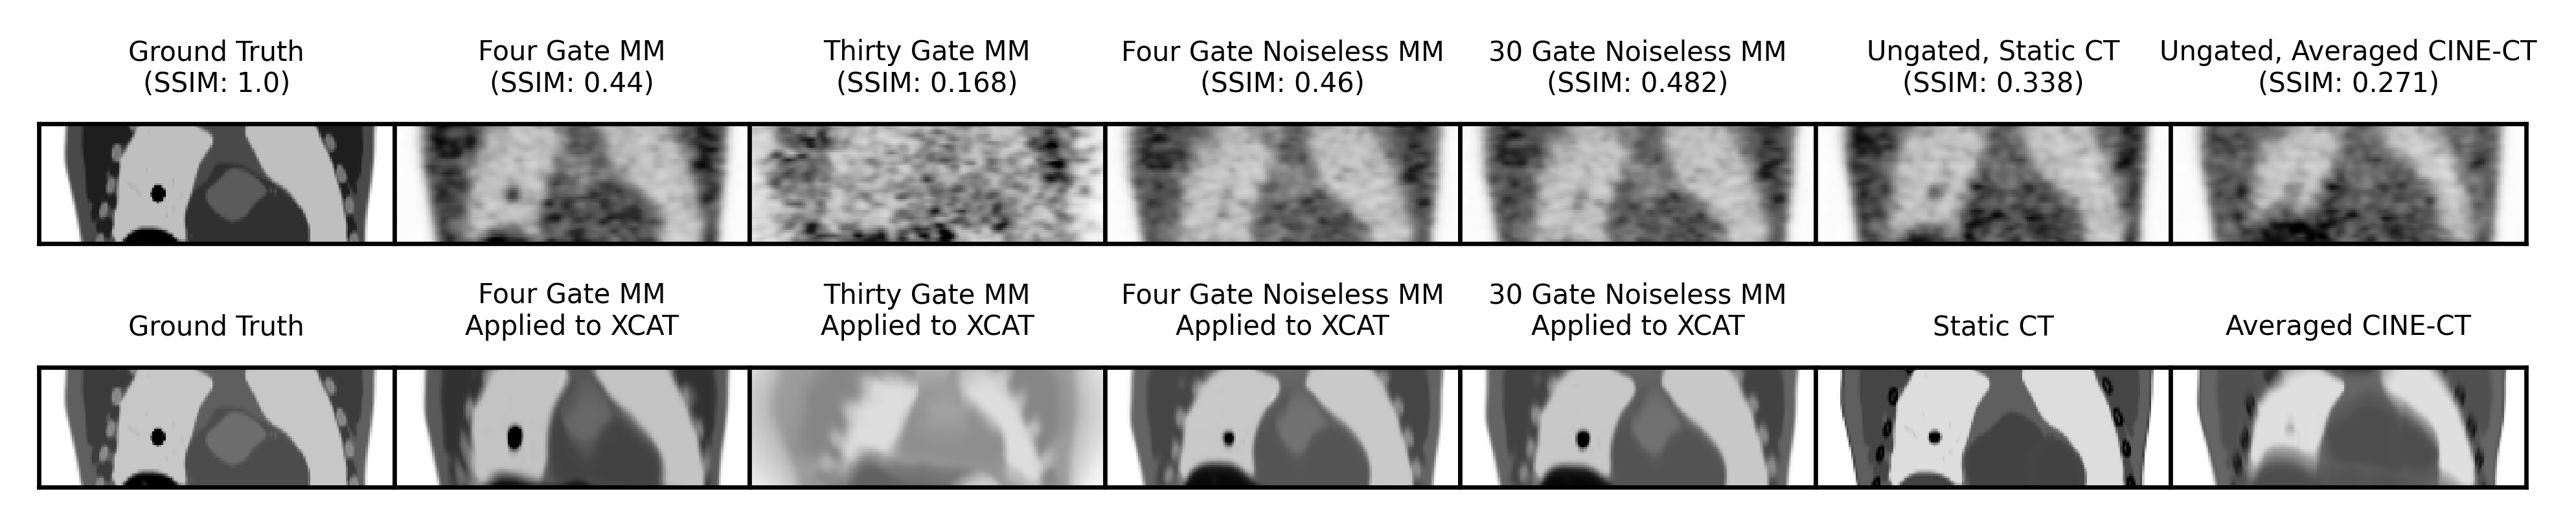
\includegraphics[width=1.0\linewidth]{figures/motion_correction_2_results_1_visual_analysis.png}
                
                \captionsetup{singlelinecheck=false}
                \caption{
                    First row contains, \gls{AC} motion corrected reconstructions (plus \gls{SSIM} to the ground truth). Second row contains, the results of applying the final \gls{MM} on the original \gls{XCAT} volumes, with the ground truth \gls{XCAT} data (for both activity and attenuation). This is using a \gls{MM} fit on four and $30$ gate binned data applied to $30$ gate binned data, a \gls{MM} fit on noiseless four and $30$ gate binned data applied to $30$ gate binned data, and ungated data \gls{AC} with a static \gls{Mu-Map} at end inhalation and all \glspl{Mu-Map} summed. Colour map ranges are consistent for all images in each row.
                }
                
                \label{fig:pet_ct_motion_correction_exploiting_motion_models_fit_on_coarsely_gated_data_applied_to_finely_gated_data_results_visual_analysis}
            \end{figure}
            
            \begin{figure}
                \centering
                
                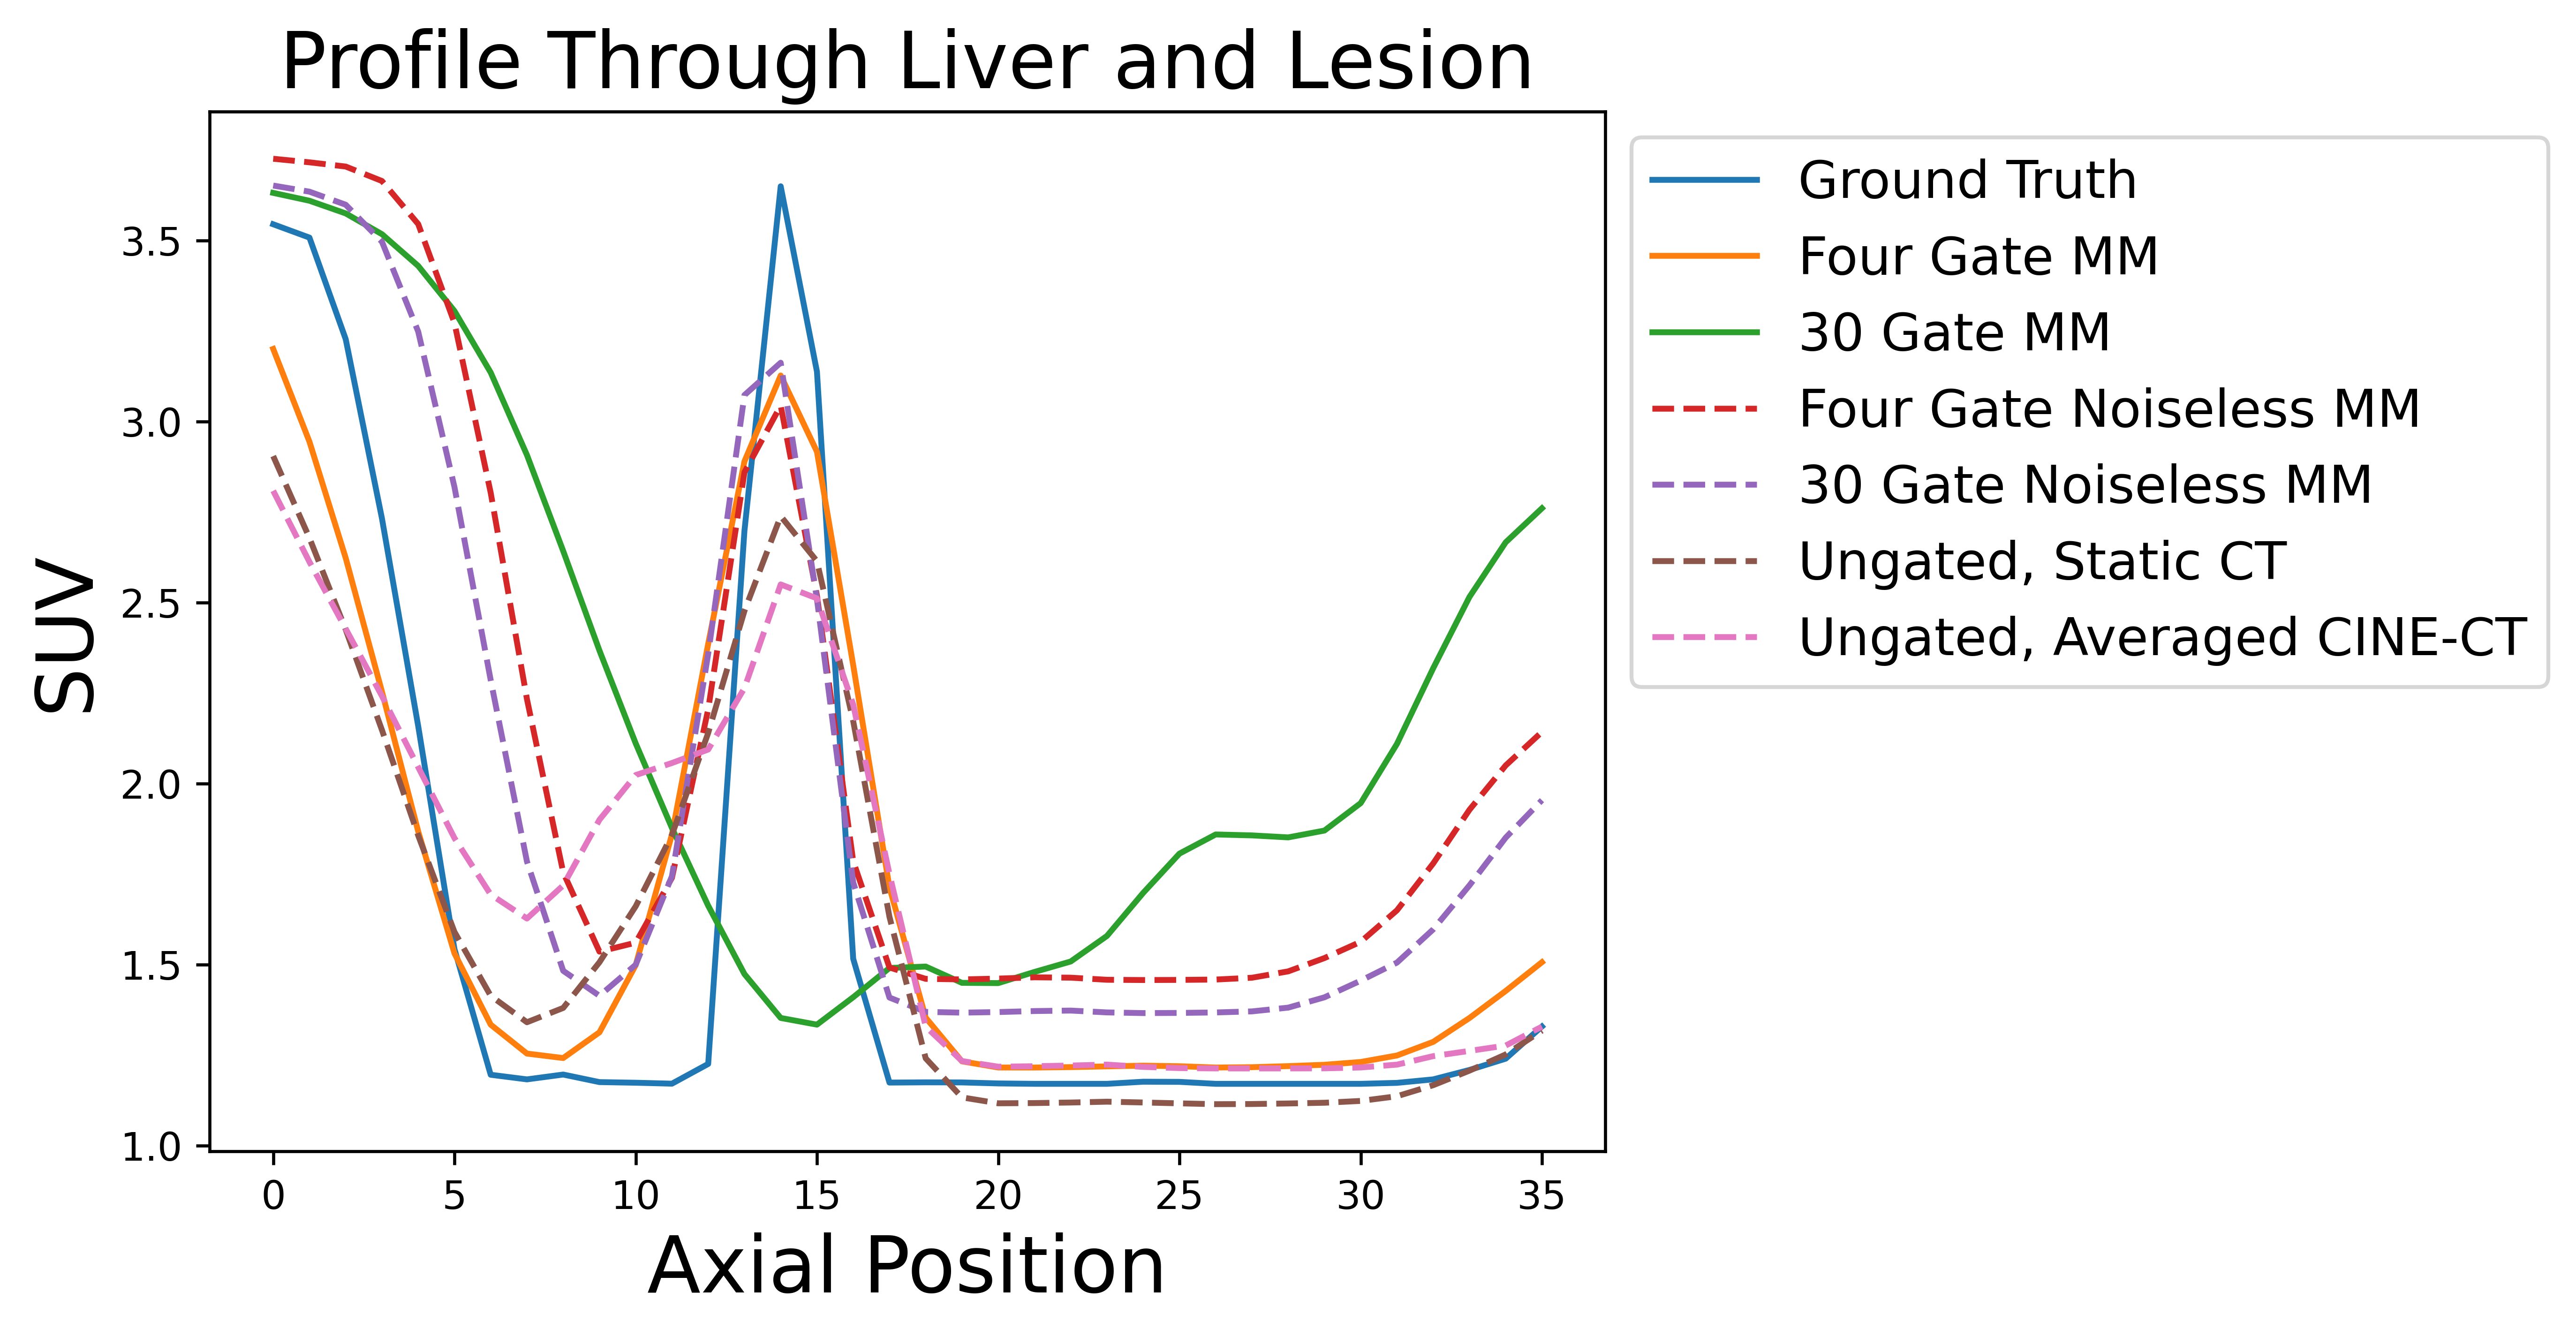
\includegraphics[width=1.0\linewidth]{figures/motion_correction_2_results_1_profile.png}
                
                \captionsetup{singlelinecheck=false}
                \caption{
                    A profile through the lesion, in the \gls{SI} direction, summed over a window in the \gls{AP} and \gls{LM} directions, with median smoothing, for the ground truth \gls{XCAT} data, a \gls{MM} fit on four and $30$ gate binned data applied to $30$ gate binned data, a \gls{MM} fit on noiseless four and $30$ gate binned data applied to $30$ gate binned data, and ungated data \gls{AC} with a static \gls{Mu-Map} at end inhalation and all \glspl{Mu-Map} summed.
                }
                
                \label{fig:pet_ct_motion_correction_exploiting_motion_models_fit_on_coarsely_gated_data_applied_to_finely_gated_data_results_profile}
            \end{figure}
            
            \begin{table}
                \centering
                
                \captionsetup{singlelinecheck=false}
                \caption{
                    Comparison of \gls{SUV}\textsubscript{max} and \gls{SUV}\textsubscript{peak}, for the ground truth \gls{XCAT} data, a \gls{MM} fit on four and $30$ gate binned data applied to $30$ gate binned data, a \gls{MM} fit on noiseless four and $30$ gate binned data applied to $30$ gate binned data, and ungated data \gls{AC} with a static \gls{Mu-Map} at end inhalation and all \glspl{Mu-Map} summed.
                }
                
                \resizebox*{1.0\linewidth}{!}
                {
                    \begin{tabular}{||c|cc||}
                        \hline
                        \textbf{\gls{SUV}}                      & \textbf{Max}  & \textbf{Peak} \\
                        \hline
                        \textbf{Ground Truth}                   & $8.76$        & $7.96$ \\
                        \hline
                        \textbf{Four Gate \gls{MM}}             & $8.04$        & $6.18$ \\
                        \textbf{$30$ Gate \gls{MM}}             & $1.77$        & $1.32$ \\
                        \hline
                        \textbf{Four Gate Noiseless \gls{MM}}   & $8.05$        & $6.24$ \\
                        \textbf{$30$ Gate Noiseless \gls{MM}}   & $7.96$        & $5.99$ \\
                        \hline
                        \textbf{Ungated, Static \gls{CT}}       & $6.61$        & $5.08$ \\
                        \textbf{Ungated, \gls{AV-CCT}}          & $5.65$        & $4.44$ \\
                        \hline
                    \end{tabular}
                }
                \label{tab:pet_ct_motion_correction_exploiting_motion_models_fit_on_coarsely_gated_data_applied_to_finely_gated_data_results_suv}
            \end{table}
            
            A visual comparison of the reconstructed images (see~\Fref{fig:pet_ct_motion_correction_exploiting_motion_models_fit_on_coarsely_gated_data_applied_to_finely_gated_data_results_visual_analysis}), shows that the high noise high temporal/gate resolution method performs quite poorly, most probably due to the high level of noise apparent in the volumes. Conversely, the low noise low temporal/gate resolution data method appears to be able to motion correct the data without being too adversely affected by the noise level.
             
            The peak of the profile (see~\Fref{fig:pet_ct_motion_correction_exploiting_motion_models_fit_on_coarsely_gated_data_applied_to_finely_gated_data_results_profile}) for the four gate \gls{MM} results is comparable to the noiseless results. In contrast, the $30$ gate \gls{MM} method fails on the noisy data. For all other motion correction methods, the peak is greater than without motion correction.
             
            \gls{SUV} (and \gls{SSIM}) results confirm the above (see~\Fref{tab:pet_ct_motion_correction_exploiting_motion_models_fit_on_coarsely_gated_data_applied_to_finely_gated_data_results_suv}).

        \subsection{Conclusion} \label{sec:pet_ct_motion_correction_exploiting_motion_models_fit_on_coarsely_gated_data_applied_to_finely_gated_data_conclusion}
            Results show that using a low number of gates for \gls{MM} fitting, has minimal impact at low noise, while improving motion correction when there is a high level of noise in the gates. In addition, the execution time using a reduced number of gates is lower.
            
            In the future, work will focus on evaluating the method on patient data.

    \section{Evaluation of PET/CT Motion Correction Incorporating Motion Models Using MLACF and Complex Gating Schemes} \label{sec:evaluation_of_pet_ct_motion_correction_incorporating_motion_models_using_mlacf_and_complex_gating_schemes}
        This section demonstrates work performed in order to prepare the methods presented previously to the application of patient data. Furthermore, it highlights the benefits of using \gls{MLACF} during motion correction and also proposes an argument for \gls{2D} gating.

        \subsection{Introduction} \label{sec:evaluation_of_pet_ct_motion_correction_incorporating_motion_models_using_mlacf_and_complex_gating_schemes_introduction}
            This work functions as a companion piece to~\Fref{sec:pet_ct_motion_correction_exploiting_motion_models_fit_on_coarsely_gated_data_applied_to_finely_gated_data}. The methods presented here do not differ significantly from those shown before. Where not otherwise stated, it can be assumed that the methods used here followed~\Fref{sec:pet_ct_motion_correction_exploiting_motion_models_fit_on_coarsely_gated_data_applied_to_finely_gated_data}. However, there were large strides made to prepare the method for use with patient data. These include making the simulation data as similar to \gls{GE} Discovery $710$ patient data as possible, as well as testing but not evaluating the method using the same data. Moreover, some improvements to the general implementation of the method are also presented. For instance, \gls{MLACF} was made more robust and stable, compared to what was used in~\Fref{sec:pet_ct_motion_correction_exploiting_motion_models_fit_on_coarsely_gated_data_applied_to_finely_gated_data}. Additionally, the parameters of the method were optimised using a grid search. Furthermore, an evaluation of the impact of including \gls{MLACF} and \gls{2D} \glspl{SS} is also shown.
        
        \subsection{Methods} \label{sec:evaluation_of_pet_ct_motion_correction_incorporating_motion_models_using_mlacf_and_complex_gating_schemes_methods}
            \gls{AC} volumes are reconstructed using \gls{MLACF} (also using \gls{AC} and \gls{NAC} \gls{OSEM}) with improvements for stability (`phase' gated into three, four, eight, and $12$ bins and amplitude gated into five and $30$ bins), as seen in~\Fref{sec:evaluation_of_pet_ct_motion_correction_incorporating_motion_models_using_mlacf_and_complex_gating_schemes_methods_xcat_volume_generation_and_pet_acquisition_simulation} and~\Fref{sec:evaluation_of_pet_ct_motion_correction_incorporating_motion_models_using_mlacf_and_complex_gating_schemes_methods_image_reconstruction}. These volumes are taken as input for a pyramidical group-wise registration and \gls{MM} estimation. The reference \gls{PET} volume, from the previous step, is registered at each iteration to a single \gls{Mu-Map}, at end inhalation. The resultant \gls{MM} and its inverse are used to perform a motion compensated \gls{AC} reconstruction, all as seen in~\Fref{sec:evaluation_of_pet_ct_motion_correction_incorporating_motion_models_using_mlacf_and_complex_gating_schemes_methods_registration_motion_model_estimation_and_motion_corrected_image_reconstruction_with_attenuation_correction}.
            
            For validation, \gls{XCAT} simulations are used, for one bed position, with a \gls{FOV} including the base of the lungs and the diaphragm. The output for data `phase' gated into three, four, eight, and $12$ and amplitude gated into five and $30$ bins are evaluated against the following. Firstly, a ground truth \gls{XCAT} volume. Secondly, a non-motion corrected reconstruction of the same data (using a single static \gls{Mu-Map} for attenuation correction). Evaluations performed included a visual analysis (\gls{PIQE}), an examination of profile, and \gls{SUV} analysis, shown in~\Fref{sec:evaluation_of_pet_ct_motion_correction_incorporating_motion_models_using_mlacf_and_complex_gating_schemes_methods_evaluation}.
            
            \subsubsection{XCAT Volume Generation and PET Acquisition Simulation} \label{sec:evaluation_of_pet_ct_motion_correction_incorporating_motion_models_using_mlacf_and_complex_gating_schemes_methods_xcat_volume_generation_and_pet_acquisition_simulation}
                \gls{XCAT} volumes were acquired in the same way as in~\Fref{sec:pet_ct_motion_correction_exploiting_motion_models_fit_on_coarsely_gated_data_applied_to_finely_gated_data_methods_xcat_volume_generation}.

                \gls{PET} acquisitions were simulated (and reconstructed) similarly to in~\Fref{sec:pet_ct_motion_correction_exploiting_motion_models_fit_on_coarsely_gated_data_applied_to_finely_gated_data_methods_pet_acquisition_simulation}. However, a great deal of care was taken to ensure the simulated data matched real \gls{GE} Discovery $710$ patient data as closely as possible. Count levels were set to those from a research study (which used the \gls{GE} Discovery $710$). The \gls{TOF} resolution used for simulation was the same as the \gls{GE} Discovery $710$ \gls{PET}/\gls{CT}, rather than the improved \gls{TOF} resolution from the \gls{GE} Signa \gls{PET}/\gls{MR} (as was used in all previous work). Pseudo-randoms and scatter were added in a similar way as in~\Fref{sec:pet_ct_motion_correction_exploiting_motion_models_fit_on_coarsely_gated_data_applied_to_finely_gated_data_methods_pet_acquisition_simulation}. However, their profile was made to match exactly the profile of randoms and scatter from the same research study as the counts. Furthermore, for the first time, \gls{3D} acquisition data was used rather than \gls{2D}. The change to \gls{3D} acquisition data may seem negligible for the evaluation of a motion correction algorithm, however, when \gls{MLACF} is introduced, the change to \gls{3D} data becomes more significant. Previously, \gls{2D} simulations and reconstruction were used purely for computational efficiency. A further addition made to increase compatibility with patient data was testing the method with randoms, scatter, and normalisation correction sinograms as a further input. The most obvious reasons for taking such care to match real \gls{GE} Discovery $710$ patient data aside, if the simulations match this data, then the likelihood of the method working for patient data is increased.
                
                A respiratory \gls{SS} was generated employing \gls{PCA}~\parencite{Thielemans2011}. The value of this signal, and its gradient, was used for gating (where appropriate). Multiple gating schemes were utilised for \gls{MM} estimation. These gating schemes were as follows.

                \begin{itemize}
                    \item `Phase' gating follows the same scheme as used in~\Fref{sec:pet_ct_motion_correction_exploiting_motion_models_fit_on_coarsely_gated_data_applied_to_finely_gated_data_methods_pet_acquisition_simulation}. In the case of Four Phase, the data was displacement and gradient gated into four bins, where each bin was a quadrant centred on the maximum or minimum of the displacement or gradient. However, there do not necessarily have to be exactly four bins. Thus, for Eight Phase and Twelve Phase it is as if each quadrant from Four Phase is split equally into two or three further bins respectively. For Three Phase the `circle' of the \gls{2D} \gls{SS} is instead split into three one third sectors (or 120 degree sectors).

                    \item Amplitude gating follows the same scheme as used in~\Fref{sec:comparison_of_motion_correction_methods_incorporating_motion_modelling_for_pet_ct_using_a_single_breath_hold_attenuation_map_pet_acquisition_simulation_and_non_attenuation_corrected_image_reconstruction}. In the case of Thirty Amplitude, the magnitude of the \gls{SS} and its gradient, was used to gate data into $30$ respiratory bins using displacement gating ($10$ amplitude and three gradient bins). In the case of Five Amplitude, five respiratory bins were used (five amplitude and one gradient bin). For Five Amplitude both a \gls{2D} and \gls{1D} \gls{SS} was used. The \gls{2D} \gls{SS} was utilised to mimic Thirty Amplitude. However, in the Five Amplitude, case only one gradient bin was used. Thus, the mean value for the gradient bin was used for each displacement bin in the Five Amplitude \gls{2D} case. In the Five Amplitude \gls{1D} case the gradient value was set to zero for each displacement bin. This is the most simple and fair way to implement a \gls{1D} \gls{SS}, however, this does mean that the \gls{MM} regression has an additional degree of freedom.
                \end{itemize}
                
            \subsubsection{Image Reconstruction} \label{sec:evaluation_of_pet_ct_motion_correction_incorporating_motion_models_using_mlacf_and_complex_gating_schemes_methods_image_reconstruction}
                \gls{MLACF} reconstruction mainly followed~\Fref{sec:pet_ct_motion_correction_exploiting_motion_models_fit_on_coarsely_gated_data_applied_to_finely_gated_data_methods_mlacf_image_reconstruction}. Three full iterations and $24$ subsets for the activity update, and one iteration for the attenuation update were used~\parencite{Nuyts2012ML-reconstructionFactors}. One iteration for the attenuation update was found to be sufficient. This is the case because the first update of the \glspl{ACF} was large and subsequent updates were small. More iterations of activity and attenuation could be performed, in less time, if fewer updates of the \glspl{ACF} were used.
                
                Both the activity volume and \glspl{ACF} were initialised using the breath hold \gls{CT}, expecting that for the anatomy of the activity volume the breath hold \gls{CT} would be similar. However, obviously the scale and specific values would be wrong. Although, as mentioned previously, the scale of the output from \gls{MLACF} (and \gls{MLAA}) is arbitrary anyway. Both of these initialisations gave a small improvement to results without introducing bias. Between iterations, the scale of the \gls{ACF} sinogram was set to the scale of the original breath hold \gls{CT} \gls{ACF}, this in order to aid with stabilising the reconstruction. This is similar to work which (was performed simultaneously with this work) where two \glspl{ACF} were used. One \gls{ACF} was from, for instance, a  breath hold \gls{CT} and the second \gls{ACF} was the one updated by \gls{MLACF}. This second \gls{ACF} acted as a correction to the first \gls{ACF}. In the other work a regularisation term was also used to keep the scale of the corrected \glspl{ACF} close to the original \glspl{ACF} while allowing some variation~\parencite{Jolivet2022JointPET}. Although the other implementation allowed the scale of the \glspl{ACF} to vary slightly, while the work here constrained it, this is not necessarily an advantage. The activity volume would experience cross talk from the \glspl{ACF} and as such could compensate for the fact that the scale of the \glspl{ACF} was fixed. Additionally, fixing the scale of the \glspl{ACF} removes a hyperparameter (and a regularisation term) which could otherwise cause instability. Regardless, the inclusion of this step, in both works, attempts to address the scale issue of the original implementation of \gls{MLACF}.
                
                To further combat the instability of the \gls{MLACF} algorithm, processing of the activity volume was performed between each iteration. The first step of this processing was the removal and reinterpolation of outlying values. This is due to the fact that outlying values were seen, between iterations, which caused the optimisation to fail. Outliers were defined as being any value outside three times the interquartile range of the data. New values were interpolated using linear interpolation. The second step was to smooth the endplanes of the activity volume, due to the endplanes exhibiting significantly more noise and outlying values than any other slice of the volume. This noise in the endplanes was most likely caused by the reduced sensitivity of the scanner in these areas. To aid in smoothing the endplanes an `endplanes' volume was created (this was a copy of the activity volume). Outliers were removed from the `endplanes' volume (in the same way as previously but using only one times the interquartile range) before a max filter was applied across each slice (with a kernel size of three). Outliers were removed again (in the same way) before the `endplanes' volume had the first and last slice removed and then the volume, as a whole, was resampled (using linear interpolation) to the same size as the activity volume. The `endplanes' volume was then summed with the activity volume using a ramp filter for the first and last five slices. The final step of the processing was to apply median filtering, in order to promote smoothness of the activity volume.

                Reconstructions were also performed in the same way as in~\Fref{sec:initial_motion_correction_using_basic_reconstruction_and_gating_methods_with_less_challenging_data}. \gls{AC} and \gls{NAC} \gls{OSEM} (using the breath hold \gls{CT}) were used with two full iterations and $24$ subsets~\parencite{Hudson1994}. This follows standard procedure.
                
                For the `phase' gated methods only \gls{MLACF} was used. However, for the amplitude gated methods both \gls{MLACF} and \gls{OSEM} were utilised.
            
            \subsubsection{Registration, Motion Model Estimation, and Motion Corrected Image Reconstruction with Attenuation Correction} \label{sec:evaluation_of_pet_ct_motion_correction_incorporating_motion_models_using_mlacf_and_complex_gating_schemes_methods_registration_motion_model_estimation_and_motion_corrected_image_reconstruction_with_attenuation_correction}
                Registration performed was almost identical to~\Fref{sec:pet_ct_motion_correction_exploiting_motion_models_fit_on_coarsely_gated_data_applied_to_finely_gated_data_methods_registration}, however, in this work without replication of the endplanes, smoothing, or standardisation. Instead the volume was expanded with slices filled with \glspl{NaN}. \glspl{NaN} were used, rather than replication of the endslice, because voxels filled with \glspl{NaN} would not contribute to the objective function calculation. Smoothing was found to be only detrimental to the accuracy of the registration (regularisation of the optimisation was found to be sufficient). Standardisation provided no benefit.

                Group-wise registration was also used with a pair-wise initialisation. However, in contrast to in~\Fref{sec:pet_ct_motion_correction_exploiting_motion_models_fit_on_coarsely_gated_data_applied_to_finely_gated_data_methods_registration}, the reference volume for pair-wise registration was selected by finding the minimum \gls{NMI} to the breath hold \gls{CT}. Also in contrast to in~\Fref{sec:pet_ct_motion_correction_exploiting_motion_models_fit_on_coarsely_gated_data_applied_to_finely_gated_data_methods_registration}, a pyramid approach was taken to the group-wise registration. In~\Fref{sec:pet_ct_motion_correction_exploiting_motion_models_fit_on_coarsely_gated_data_applied_to_finely_gated_data_methods_registration}, registration was applied at different resolution levels. This was done where by the \gls{CPG} initially started at a resolution of $4\times4\times4$ and was upsampled to the maximum resolution of the \gls{CPG} after subsequent iterations (motion modelling was not applied at lower resolutions). However, in this work, rather than always performing one iteration before upsampling to the next resolution level, the number of iterations was a hyperparameter of the method. Also, the \gls{MM} was fit on the \gls{CPG} at lower resolutions.
                
                The \gls{MM} was applied to the task of the final motion correction in exactly the same way as in~\Fref{sec:pet_ct_motion_correction_exploiting_motion_models_fit_on_coarsely_gated_data_applied_to_finely_gated_data_methods_mc_image_reconstruction_with_ac}.
            
            \subsubsection{Evaluation} \label{sec:evaluation_of_pet_ct_motion_correction_incorporating_motion_models_using_mlacf_and_complex_gating_schemes_methods_evaluation}
                In addition to the reconstructions performed in~\Fref{sec:evaluation_of_pet_ct_motion_correction_incorporating_motion_models_using_mlacf_and_complex_gating_schemes_methods_registration_motion_model_estimation_and_motion_corrected_image_reconstruction_with_attenuation_correction}, data were also reconstructed without motion correction, using the end inhalation \gls{Mu-Map}. For the present evaluation, the volume without motion correction was registered to the position of the end inhalation \gls{Mu-Map}. Additionally, \glspl{DVF} generated by each method were also applied to the original \gls{XCAT} volumes, for visual analysis.
                
                Comparisons made included a visual analysis, \gls{PIQE}~\parencite{Chan2000Psychovisually-basedImages}, a profile over the lesion, and \gls{SUV}\textsubscript{max}, \gls{SUV}\textsubscript{median}, and \gls{SUV}\textsubscript{peak} (defined following \gls{EANM} guidelines~\parencite{Boellaard2015FDG2.0}). \gls{PIQE} is a no-reference image quality score, which is inversely correlated to the perceptual quality of the image. A high score value indicates high perceptual quality and a low score value indicates low perceptual quality.
                
        
        \subsection{Results} \label{sec:evaluation_of_pet_ct_motion_correction_incorporating_motion_models_using_mlacf_and_complex_gating_schemes_results}
            \begin{figure}
                \centering
                
                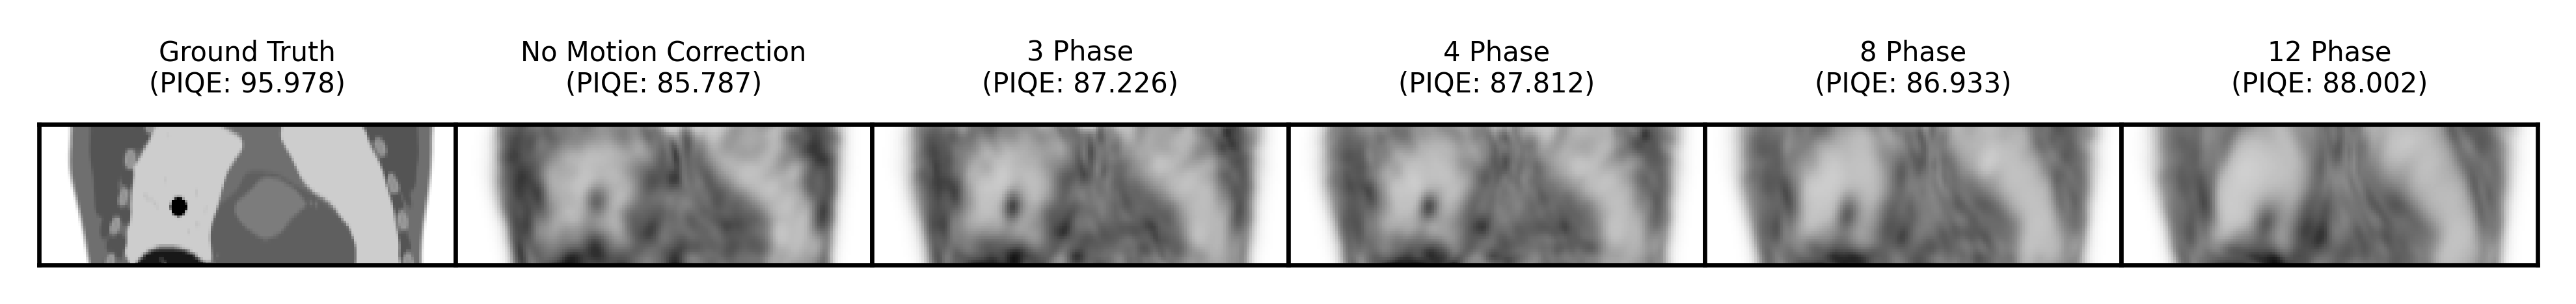
\includegraphics[width=1.0\linewidth]{figures/motion_correction_2_results_2_phase_visual_analysis.png}
                
                \captionsetup{singlelinecheck=false}
                \caption{
                    \gls{AC} motion corrected reconstructions (plus \gls{PIQE}), where different data was used to fit the \gls{MM} and the final \gls{MM} was applied to $30$ gate binned data. The data used to fit the \gls{MM} was as follows. `Phase' gated and \gls{MLACF} reconstructed data with three, four, eight and $12$ bins respectively. A \gls{MM} was also fit using a single bin, which is practically the equivalent of doing no motion correction. Colour map ranges are consistent for all images in each row.
                }
                
                \label{fig:evaluation_of_pet_ct_motion_correction_incorporating_motion_models_using_mlacf_and_complex_gating_schemes_results_phase_visual_analysis}
            \end{figure}

            \begin{figure}
                \centering
                
                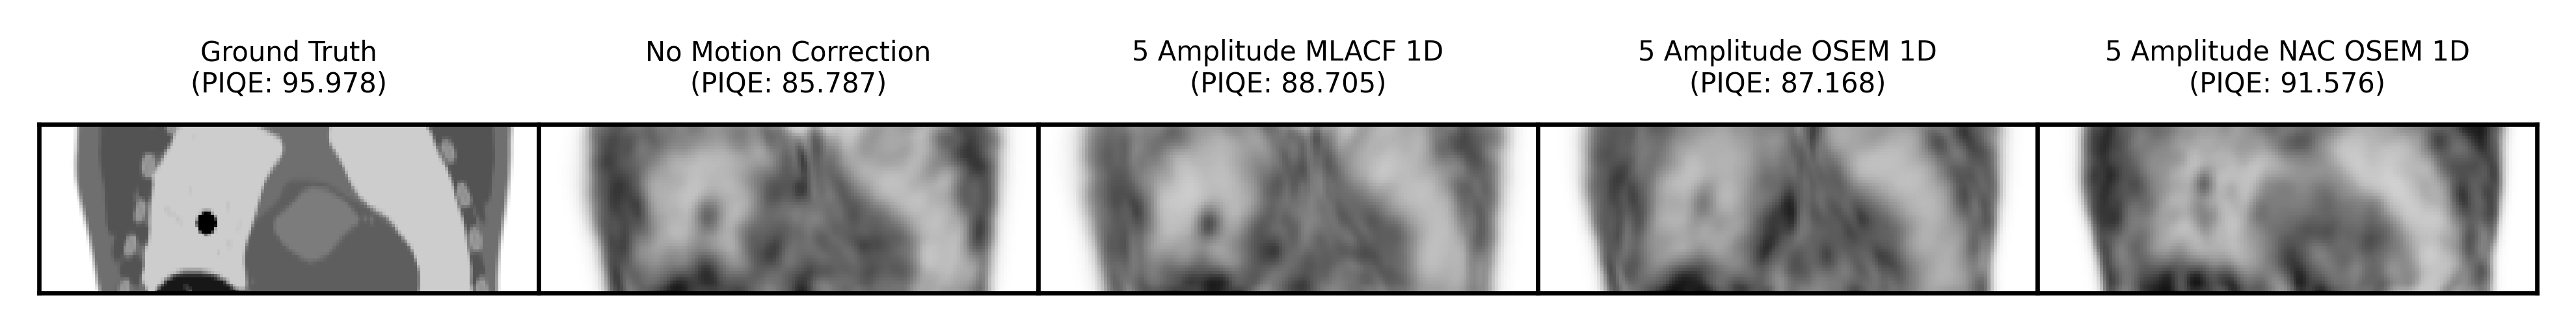
\includegraphics[width=1.0\linewidth]{figures/motion_correction_2_results_2_5_amplitude_visual_analysis.png}
                
                \captionsetup{singlelinecheck=false}
                \caption{
                    \gls{AC} motion corrected reconstructions (plus \gls{PIQE}), where different data was used to fit the \gls{MM} and the final \gls{MM} was applied to $30$ gate binned data. The data used to fit the \gls{MM} was as follows. Amplitude gated data with five bins reconstructed using \gls{MLACF}, \gls{AC} \gls{OSEM}, and \gls{NAC} \gls{OSEM}. A \gls{MM} was also fit using a single bin, which is practically the equivalent of doing no motion correction. Colour map ranges are consistent for all images in each row.
                }
                
                \label{fig:evaluation_of_pet_ct_motion_correction_incorporating_motion_models_using_mlacf_and_complex_gating_schemes_results_5_amplitude_visual_analysis}
            \end{figure}

            \begin{figure}
                \centering
                
                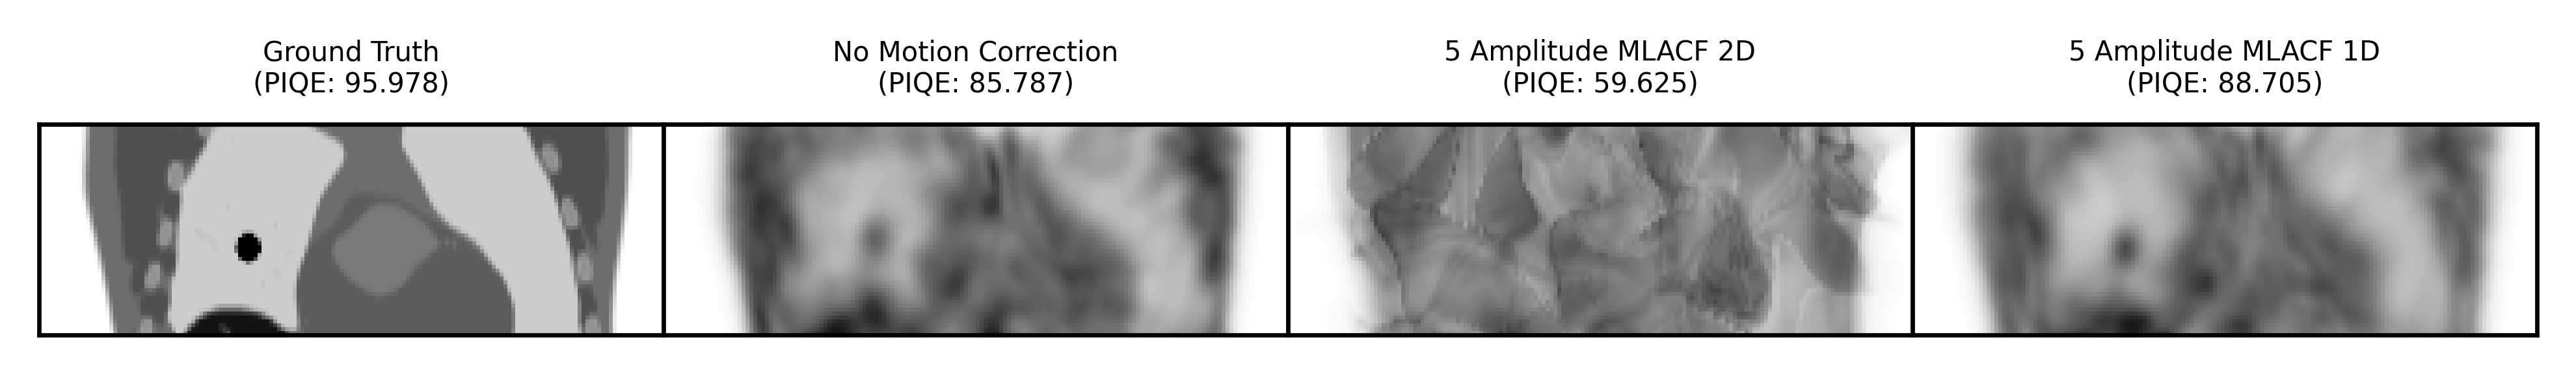
\includegraphics[width=1.0\linewidth]{figures/motion_correction_2_results_2_1d_vs_2d_visual_analysis.png}
                
                \captionsetup{singlelinecheck=false}
                \caption{
                    \gls{AC} motion corrected reconstructions (plus \gls{PIQE}), where different data was used to fit the \gls{MM} and the final \gls{MM} was applied to $30$ gate binned data. The data used to fit the \gls{MM} was as follows. Amplitude gated data with five bins reconstructed using \gls{MLACF}. Here, in the \gls{2D} case a \gls{2D} \gls{SS} and in the \gls{1D} case a \gls{1D} \gls{SS} were used. A \gls{MM} was also fit using a single bin, which is practically the equivalent of doing no motion correction. Colour map ranges are consistent for all images in each row.
                }
                
                \label{fig:evaluation_of_pet_ct_motion_correction_incorporating_motion_models_using_mlacf_and_complex_gating_schemes_results_1d_vs_2d_visual_analysis}
            \end{figure}

            \begin{figure}
                \centering
                
                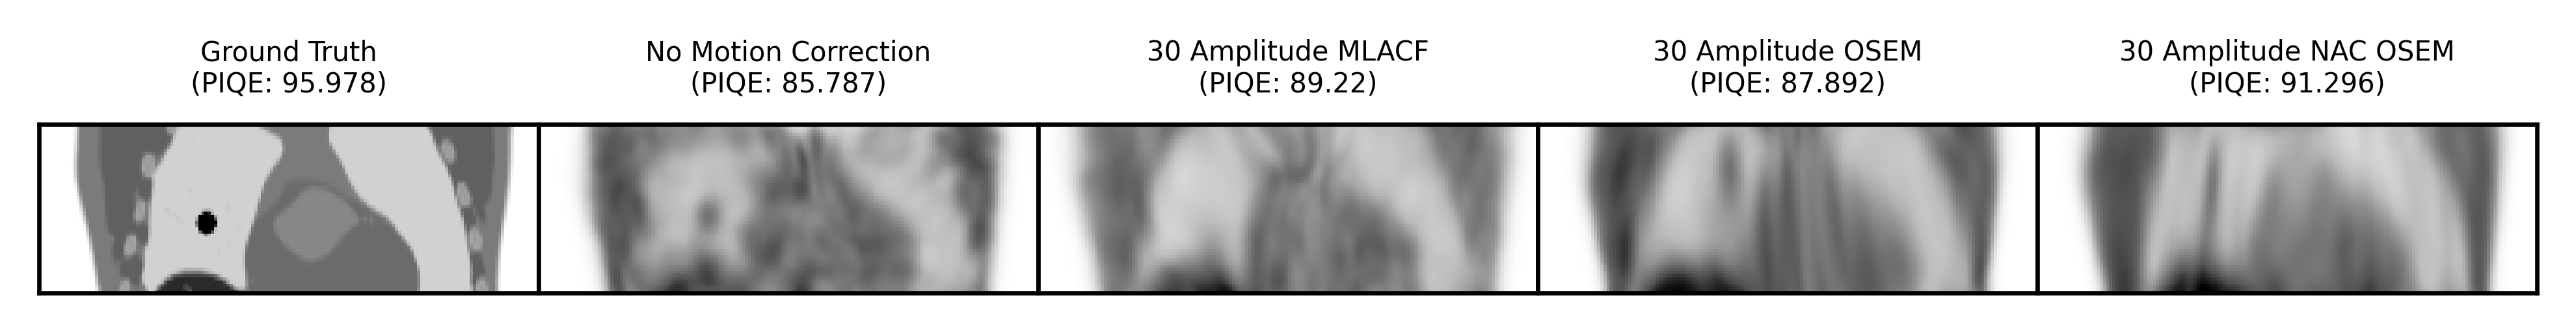
\includegraphics[width=1.0\linewidth]{figures/motion_correction_2_results_2_30_amplitude_visual_analysis.png}
                
                \captionsetup{singlelinecheck=false}
                \caption{
                    \gls{AC} motion corrected reconstructions (plus \gls{PIQE}), where different data was used to fit the \gls{MM} and the final \gls{MM} was applied to $30$ gate binned data. The data used to fit the \gls{MM} was as follows. Amplitude gated data with $30$ bins reconstructed using \gls{MLACF}, \gls{AC} \gls{OSEM}, and \gls{NAC} \gls{OSEM}. A \gls{MM} was also fit using a single bin, which is practically the equivalent of doing no motion correction. Colour map ranges are consistent for all images in each row.
                }
                
                \label{fig:evaluation_of_pet_ct_motion_correction_incorporating_motion_models_using_mlacf_and_complex_gating_schemes_results_30_amplitude_visual_analysis}
            \end{figure}

            \begin{figure}
                \centering
                
                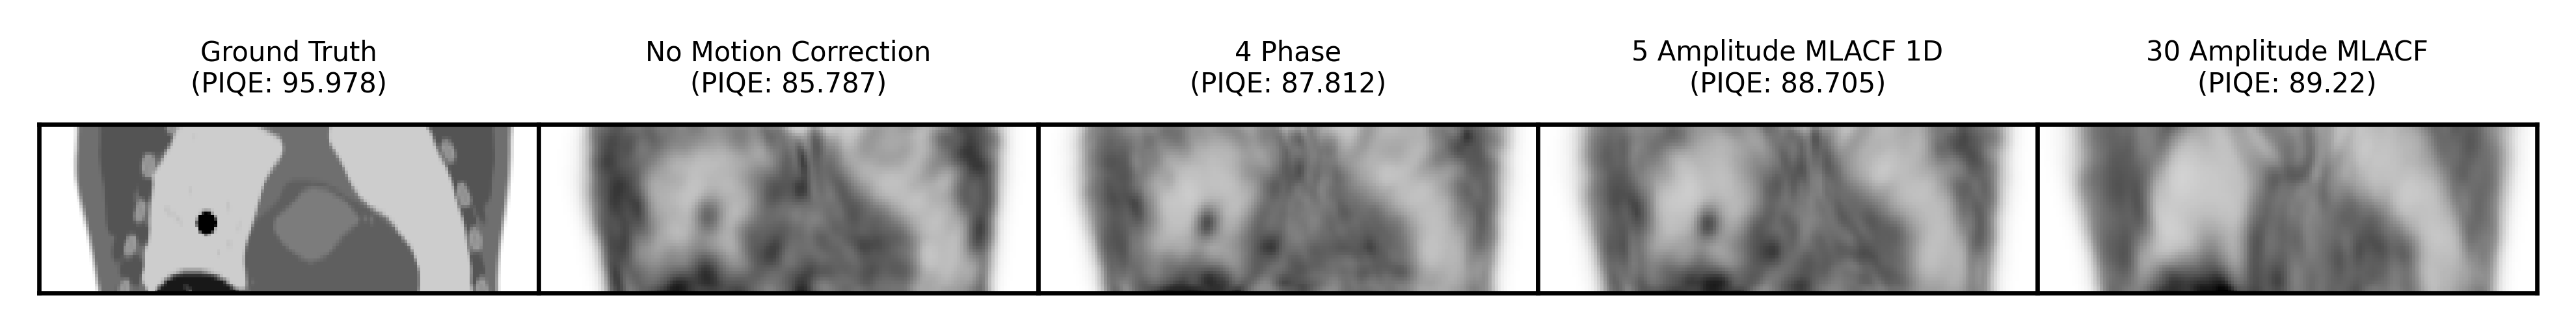
\includegraphics[width=1.0\linewidth]{figures/motion_correction_2_results_2_best_visual_analysis.png}
                
                \captionsetup{singlelinecheck=false}
                \caption{
                    \gls{AC} motion corrected reconstructions (plus \gls{PIQE}), where different data was used to fit the \gls{MM} and the final \gls{MM} was applied to $30$ gate binned data. The methods presented here are a combination of the best one method from~\Fref{fig:evaluation_of_pet_ct_motion_correction_incorporating_motion_models_using_mlacf_and_complex_gating_schemes_results_phase_visual_analysis}, ~\Fref{fig:evaluation_of_pet_ct_motion_correction_incorporating_motion_models_using_mlacf_and_complex_gating_schemes_results_5_amplitude_visual_analysis}, and~\Fref{fig:evaluation_of_pet_ct_motion_correction_incorporating_motion_models_using_mlacf_and_complex_gating_schemes_results_30_amplitude_visual_analysis}. A \gls{MM} was also fit using a single bin, which is practically the equivalent of doing no motion correction. Colour map ranges are consistent for all images in each row.
                }
                
                \label{fig:evaluation_of_pet_ct_motion_correction_incorporating_motion_models_using_mlacf_and_complex_gating_schemes_results_best_visual_analysis}
            \end{figure}
            
            \begin{figure}
                \centering
                
                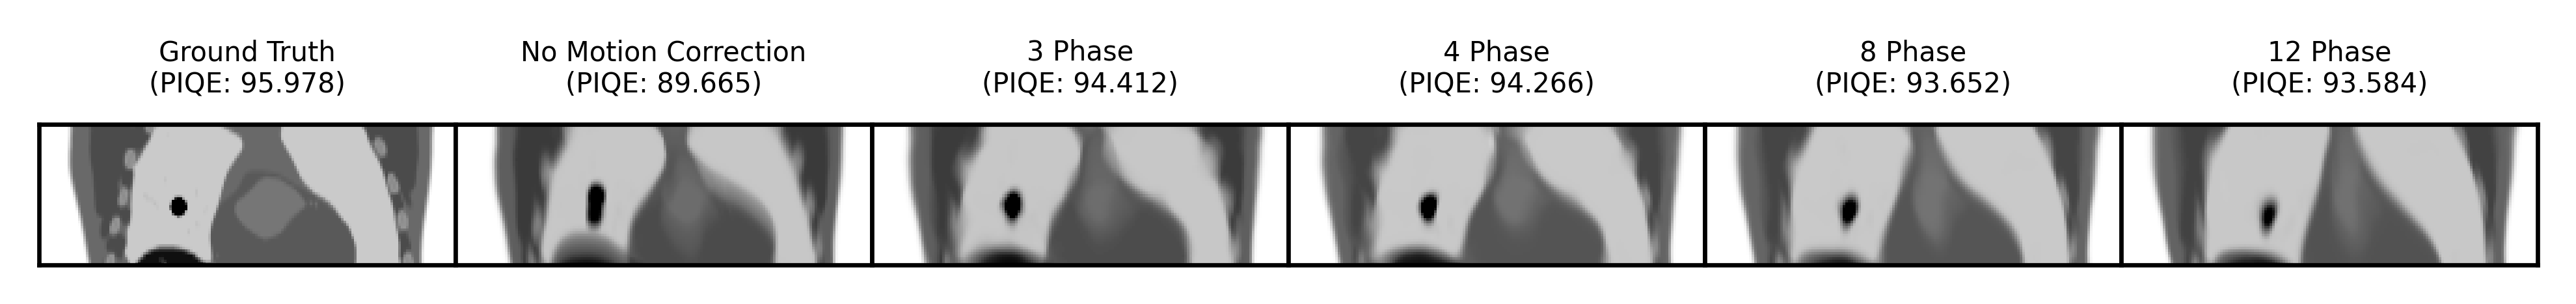
\includegraphics[width=1.0\linewidth]{figures/motion_correction_2_results_2_noiseless_phase_visual_analysis.png}
                
                \captionsetup{singlelinecheck=false}
                \caption{
                    \gls{AC} motion corrected reconstructions (plus \gls{PIQE}), where different data was used to fit the \gls{MM} and the final \gls{MM} was applied to $30$ gate binned data. The data used to fit the \gls{MM} was as follows. `Phase' gated and \gls{MLACF} reconstructed data with three, four, eight and $12$ bins respectively. A \gls{MM} was also fit using a single bin, which is practically the equivalent of doing no motion correction. Here, results are shown applied to volumes without noise. This is due to it potentially being easier to see smaller differences between motion correction methods when noise is removed. However, noise is still used during the motion correction process. Colour map ranges are consistent for all images in each row.
                }
                
                \label{fig:evaluation_of_pet_ct_motion_correction_incorporating_motion_models_using_mlacf_and_complex_gating_schemes_results_noiseless_phase_visual_analysis}
            \end{figure}

            \begin{figure}
                \centering
                
                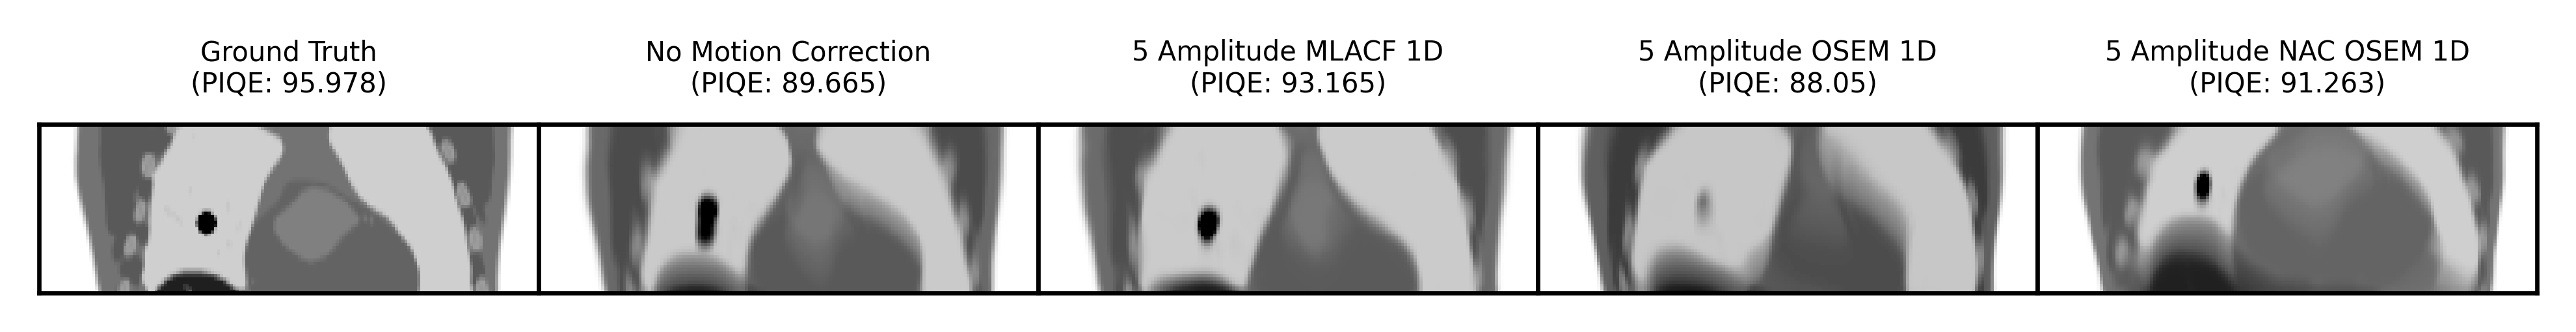
\includegraphics[width=1.0\linewidth]{figures/motion_correction_2_results_2_noiseless_5_amplitude_visual_analysis.png}
                
                \captionsetup{singlelinecheck=false}
                \caption{
                    \gls{AC} motion corrected reconstructions (plus \gls{PIQE}), where different data was used to fit the \gls{MM} and the final \gls{MM} was applied to $30$ gate binned data. The data used to fit the \gls{MM} was as follows. Amplitude gated data with five bins reconstructed using \gls{MLACF}, \gls{AC} \gls{OSEM}, and \gls{NAC} \gls{OSEM}. A \gls{MM} was also fit using a single bin, which is practically the equivalent of doing no motion correction. Here, results are shown applied to volumes without noise. This is due to it potentially being easier to see smaller differences between motion correction methods when noise is removed. However, noise is still used during the motion correction process. Colour map ranges are consistent for all images in each row.
                }
                
                \label{fig:evaluation_of_pet_ct_motion_correction_incorporating_motion_models_using_mlacf_and_complex_gating_schemes_results_noiseless_5_amplitude_visual_analysis}
            \end{figure}

            \begin{figure}
                \centering
                
                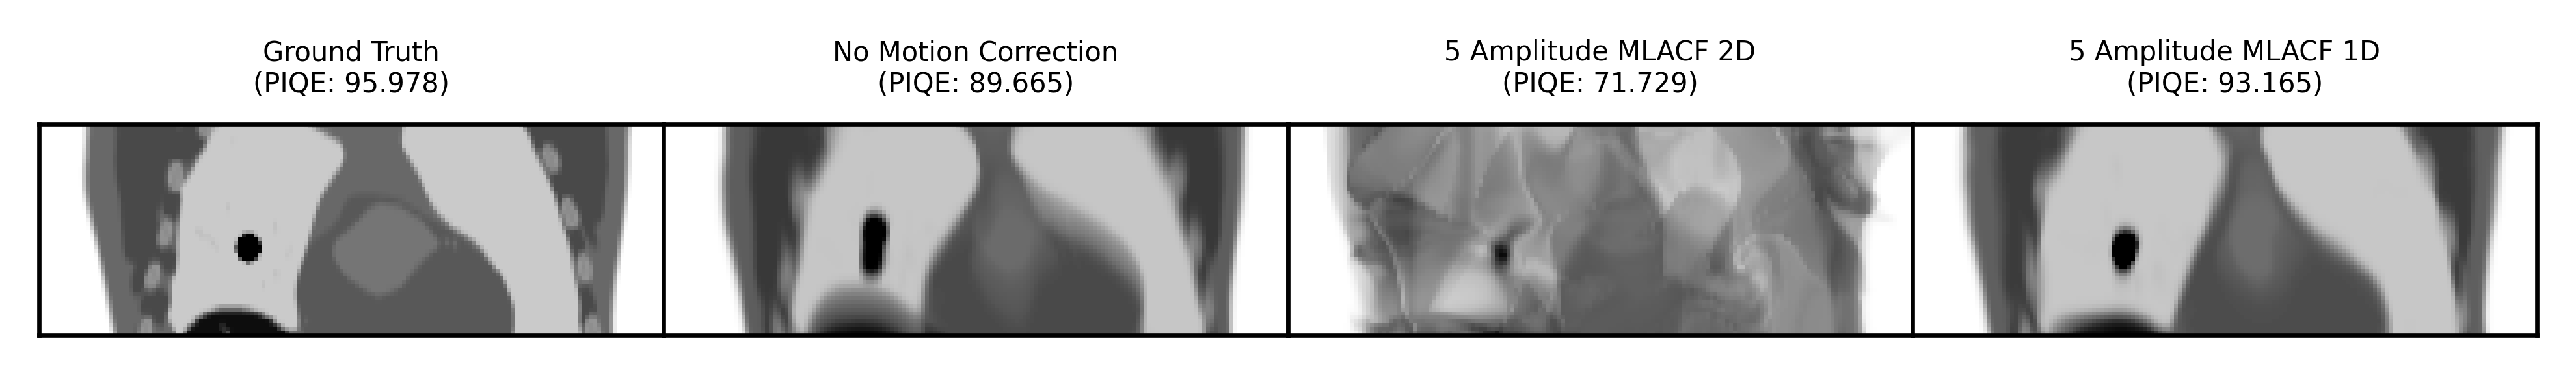
\includegraphics[width=1.0\linewidth]{figures/motion_correction_2_results_2_noiseless_1d_vs_2d_visual_analysis.png}
                
                \captionsetup{singlelinecheck=false}
                \caption{
                    \gls{AC} motion corrected reconstructions (plus \gls{PIQE}), where different data was used to fit the \gls{MM} and the final \gls{MM} was applied to $30$ gate binned data. The data used to fit the \gls{MM} was as follows. Amplitude gated data with five bins reconstructed using \gls{MLACF}. Here, in the \gls{2D} case a \gls{2D} \gls{SS} and in the \gls{1D} case a \gls{1D} \gls{SS} were used. A \gls{MM} was also fit using a single bin, which is practically the equivalent of doing no motion correction. Here, results are shown applied to volumes without noise. This is due to it potentially being easier to see smaller differences between motion correction methods when noise is removed. However, noise is still used during the motion correction process. Colour map ranges are consistent for all images in each row.
                }
                
                \label{fig:evaluation_of_pet_ct_motion_correction_incorporating_motion_models_using_mlacf_and_complex_gating_schemes_results_noiseless_1d_vs_2d_visual_analysis}
            \end{figure}

            \begin{figure}
                \centering
                
                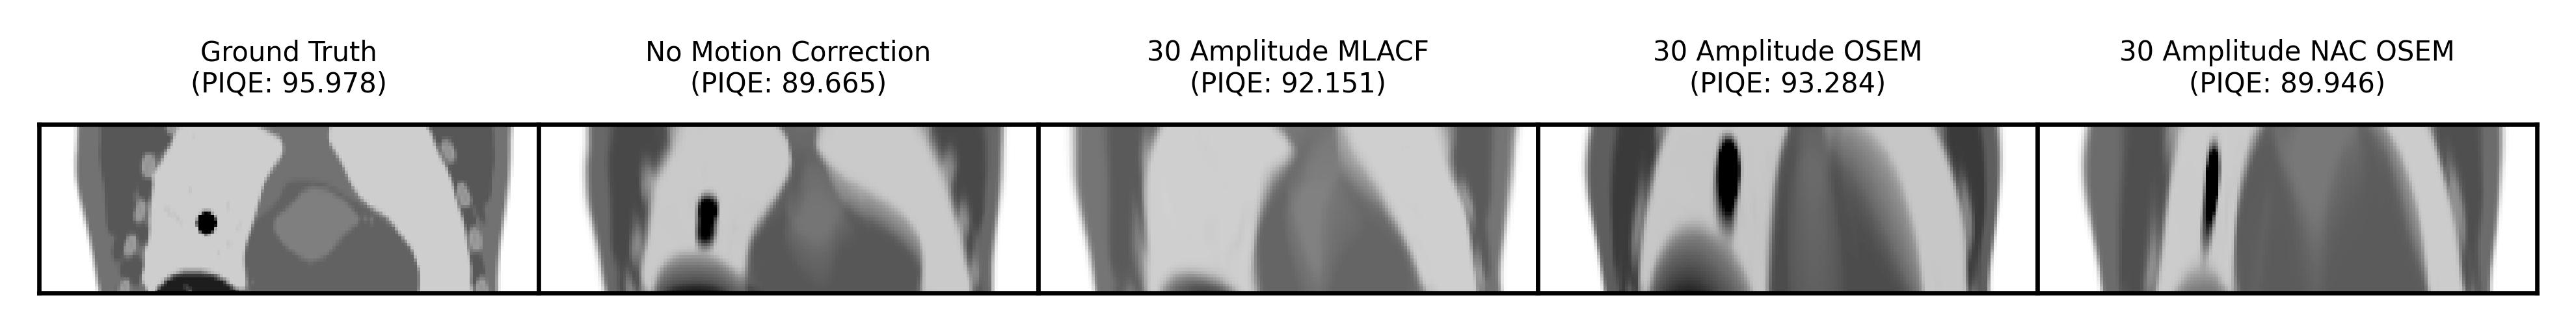
\includegraphics[width=1.0\linewidth]{figures/motion_correction_2_results_2_noiseless_30_amplitude_visual_analysis.png}
                
                \captionsetup{singlelinecheck=false}
                \caption{
                    \gls{AC} motion corrected reconstructions (plus \gls{PIQE}), where different data was used to fit the \gls{MM} and the final \gls{MM} was applied to $30$ gate binned data. The data used to fit the \gls{MM} was as follows. Amplitude gated data with $30$ bins reconstructed using \gls{MLACF}, \gls{AC} \gls{OSEM}, and \gls{NAC} \gls{OSEM}. A \gls{MM} was also fit using a single bin, which is practically the equivalent of doing no motion correction. Here, results are shown applied to volumes without noise. This is due to it potentially being easier to see smaller differences between motion correction methods when noise is removed. However, noise is still used during the motion correction process. Colour map ranges are consistent for all images in each row.
                }
                
                \label{fig:evaluation_of_pet_ct_motion_correction_incorporating_motion_models_using_mlacf_and_complex_gating_schemes_results_noiseless_30_amplitude_visual_analysis}
            \end{figure}

            \begin{figure}
                \centering
                
                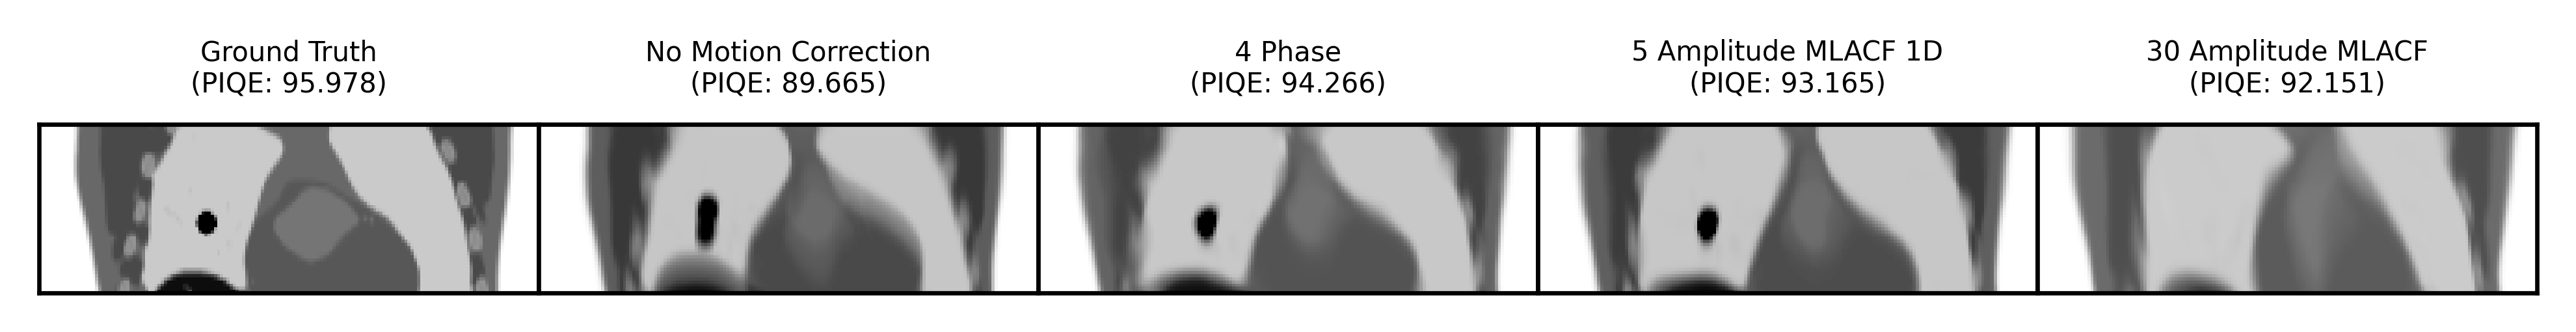
\includegraphics[width=1.0\linewidth]{figures/motion_correction_2_results_2_noiseless_best_visual_analysis.png}
                
                \captionsetup{singlelinecheck=false}
                \caption{
                    \gls{AC} motion corrected reconstructions (plus \gls{PIQE}), where different data was used to fit the \gls{MM} and the final \gls{MM} was applied to $30$ gate binned data. The methods presented here are a combination of the best one method from~\Fref{fig:evaluation_of_pet_ct_motion_correction_incorporating_motion_models_using_mlacf_and_complex_gating_schemes_results_noiseless_phase_visual_analysis}, ~\Fref{fig:evaluation_of_pet_ct_motion_correction_incorporating_motion_models_using_mlacf_and_complex_gating_schemes_results_noiseless_5_amplitude_visual_analysis}, and~\Fref{fig:evaluation_of_pet_ct_motion_correction_incorporating_motion_models_using_mlacf_and_complex_gating_schemes_results_noiseless_30_amplitude_visual_analysis}. Here, results are shown applied to volumes without noise. This is due to it potentially being easier to see smaller differences between motion correction methods when noise is removed. However, noise is still used during the motion correction process. Colour map ranges are consistent for all images in each row.
                }
                
                \label{fig:evaluation_of_pet_ct_motion_correction_incorporating_motion_models_using_mlacf_and_complex_gating_schemes_results_noiseless_best_visual_analysis}
            \end{figure}
            
            \begin{figure}
                \centering
                
                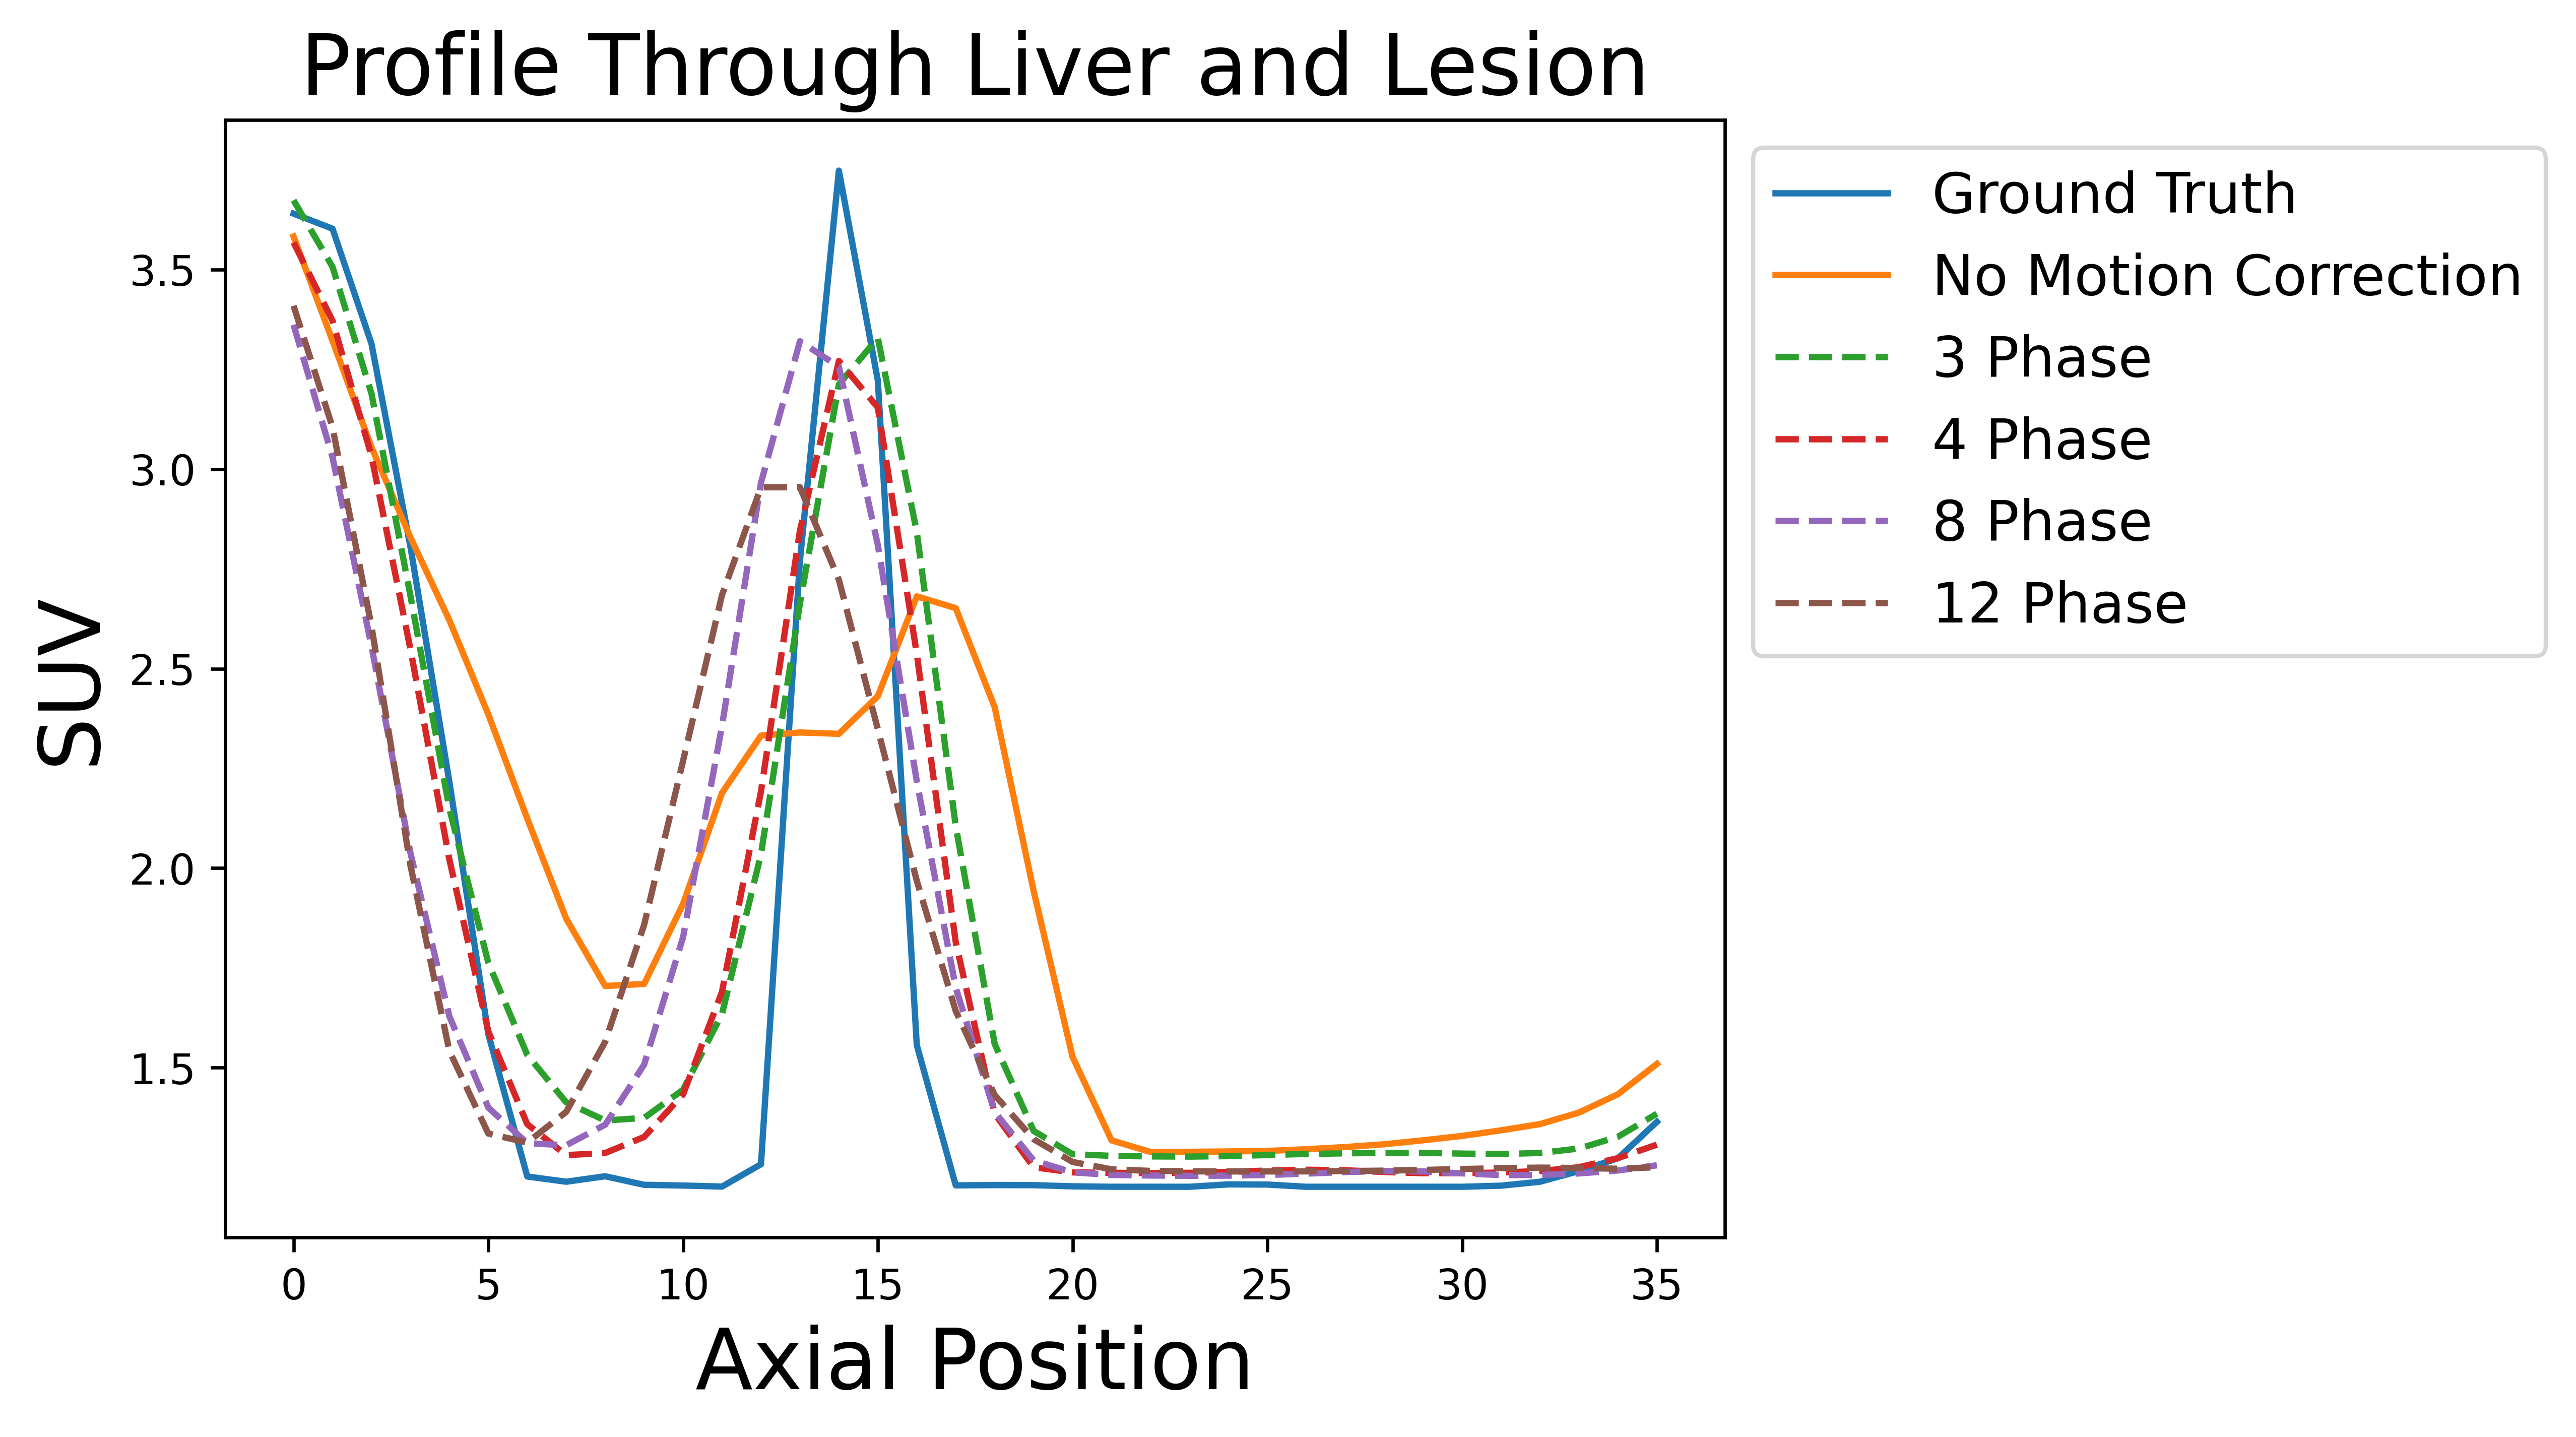
\includegraphics[width=1.0\linewidth]{figures/motion_correction_2_results_2_phase_profile.png}
                
                \captionsetup{singlelinecheck=false}
                \caption{
                    A profile through the lesion, in the \gls{SI} direction, summed over a window in the \gls{AP} and \gls{LM} directions, with median smoothing. This is for where different data was used to fit the \gls{MM} and the final \gls{MM} was applied to $30$ gate binned data. The data used to fit the \gls{MM} was as follows. `Phase' gated and \gls{MLACF} reconstructed data with three, four, eight and $12$ bins respectively. A \gls{MM} was also fit using a single bin, this is practically the equivalent of doing no motion correction.
                }
                
                \label{fig:evaluation_of_pet_ct_motion_correction_incorporating_motion_models_using_mlacf_and_complex_gating_schemes_results_phase_profile}
            \end{figure}

            \begin{figure}
                \centering
                
                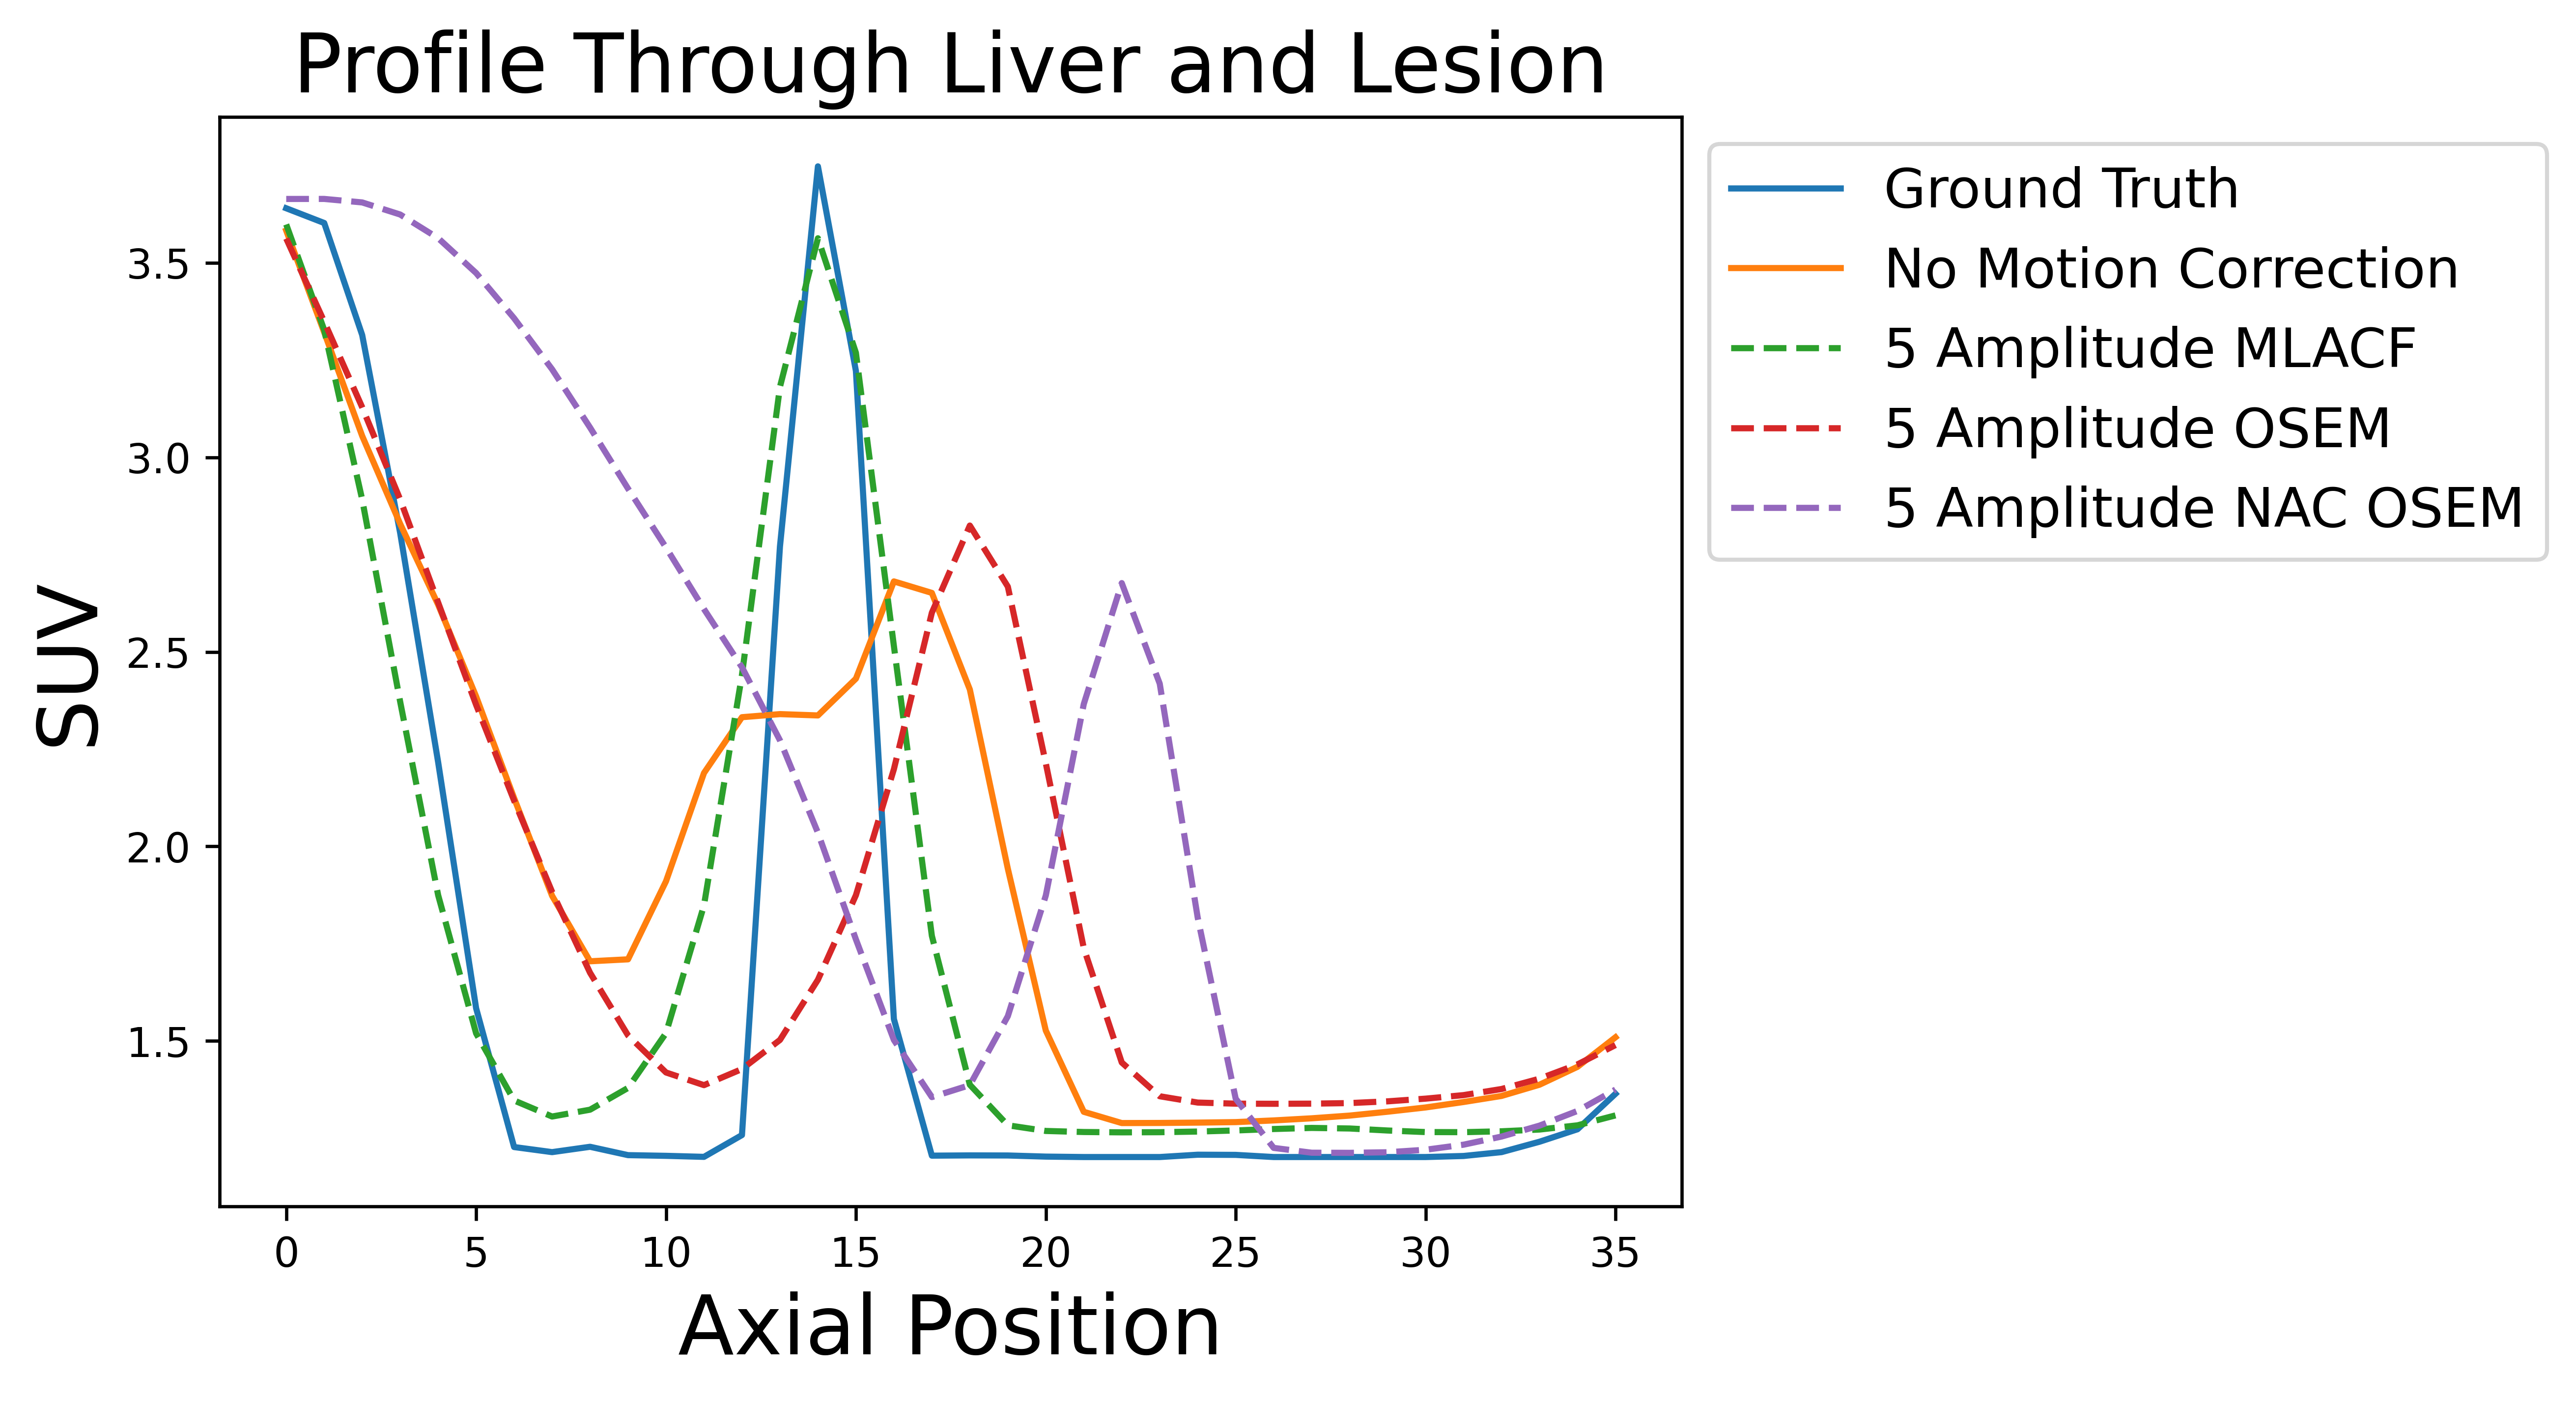
\includegraphics[width=1.0\linewidth]{figures/motion_correction_2_results_2_5_amplitude_profile.png}
                
                \captionsetup{singlelinecheck=false}
                \caption{
                    A profile through the lesion, in the \gls{SI} direction, summed over a window in the \gls{AP} and \gls{LM} directions, with median smoothing. This is for where different data was used to fit the \gls{MM} and the final \gls{MM} was applied to $30$ gate binned data. The data used to fit the \gls{MM} was as follows. Amplitude gated data with five bins reconstructed using \gls{MLACF}, \gls{AC} \gls{OSEM}, and \gls{NAC} \gls{OSEM}. A \gls{MM} was also fit using a single bin, which is practically the equivalent of doing no motion correction.
                }
                
                \label{fig:evaluation_of_pet_ct_motion_correction_incorporating_motion_models_using_mlacf_and_complex_gating_schemes_results_5_amplitude_profile}
            \end{figure}

            \begin{figure}
                \centering
                
                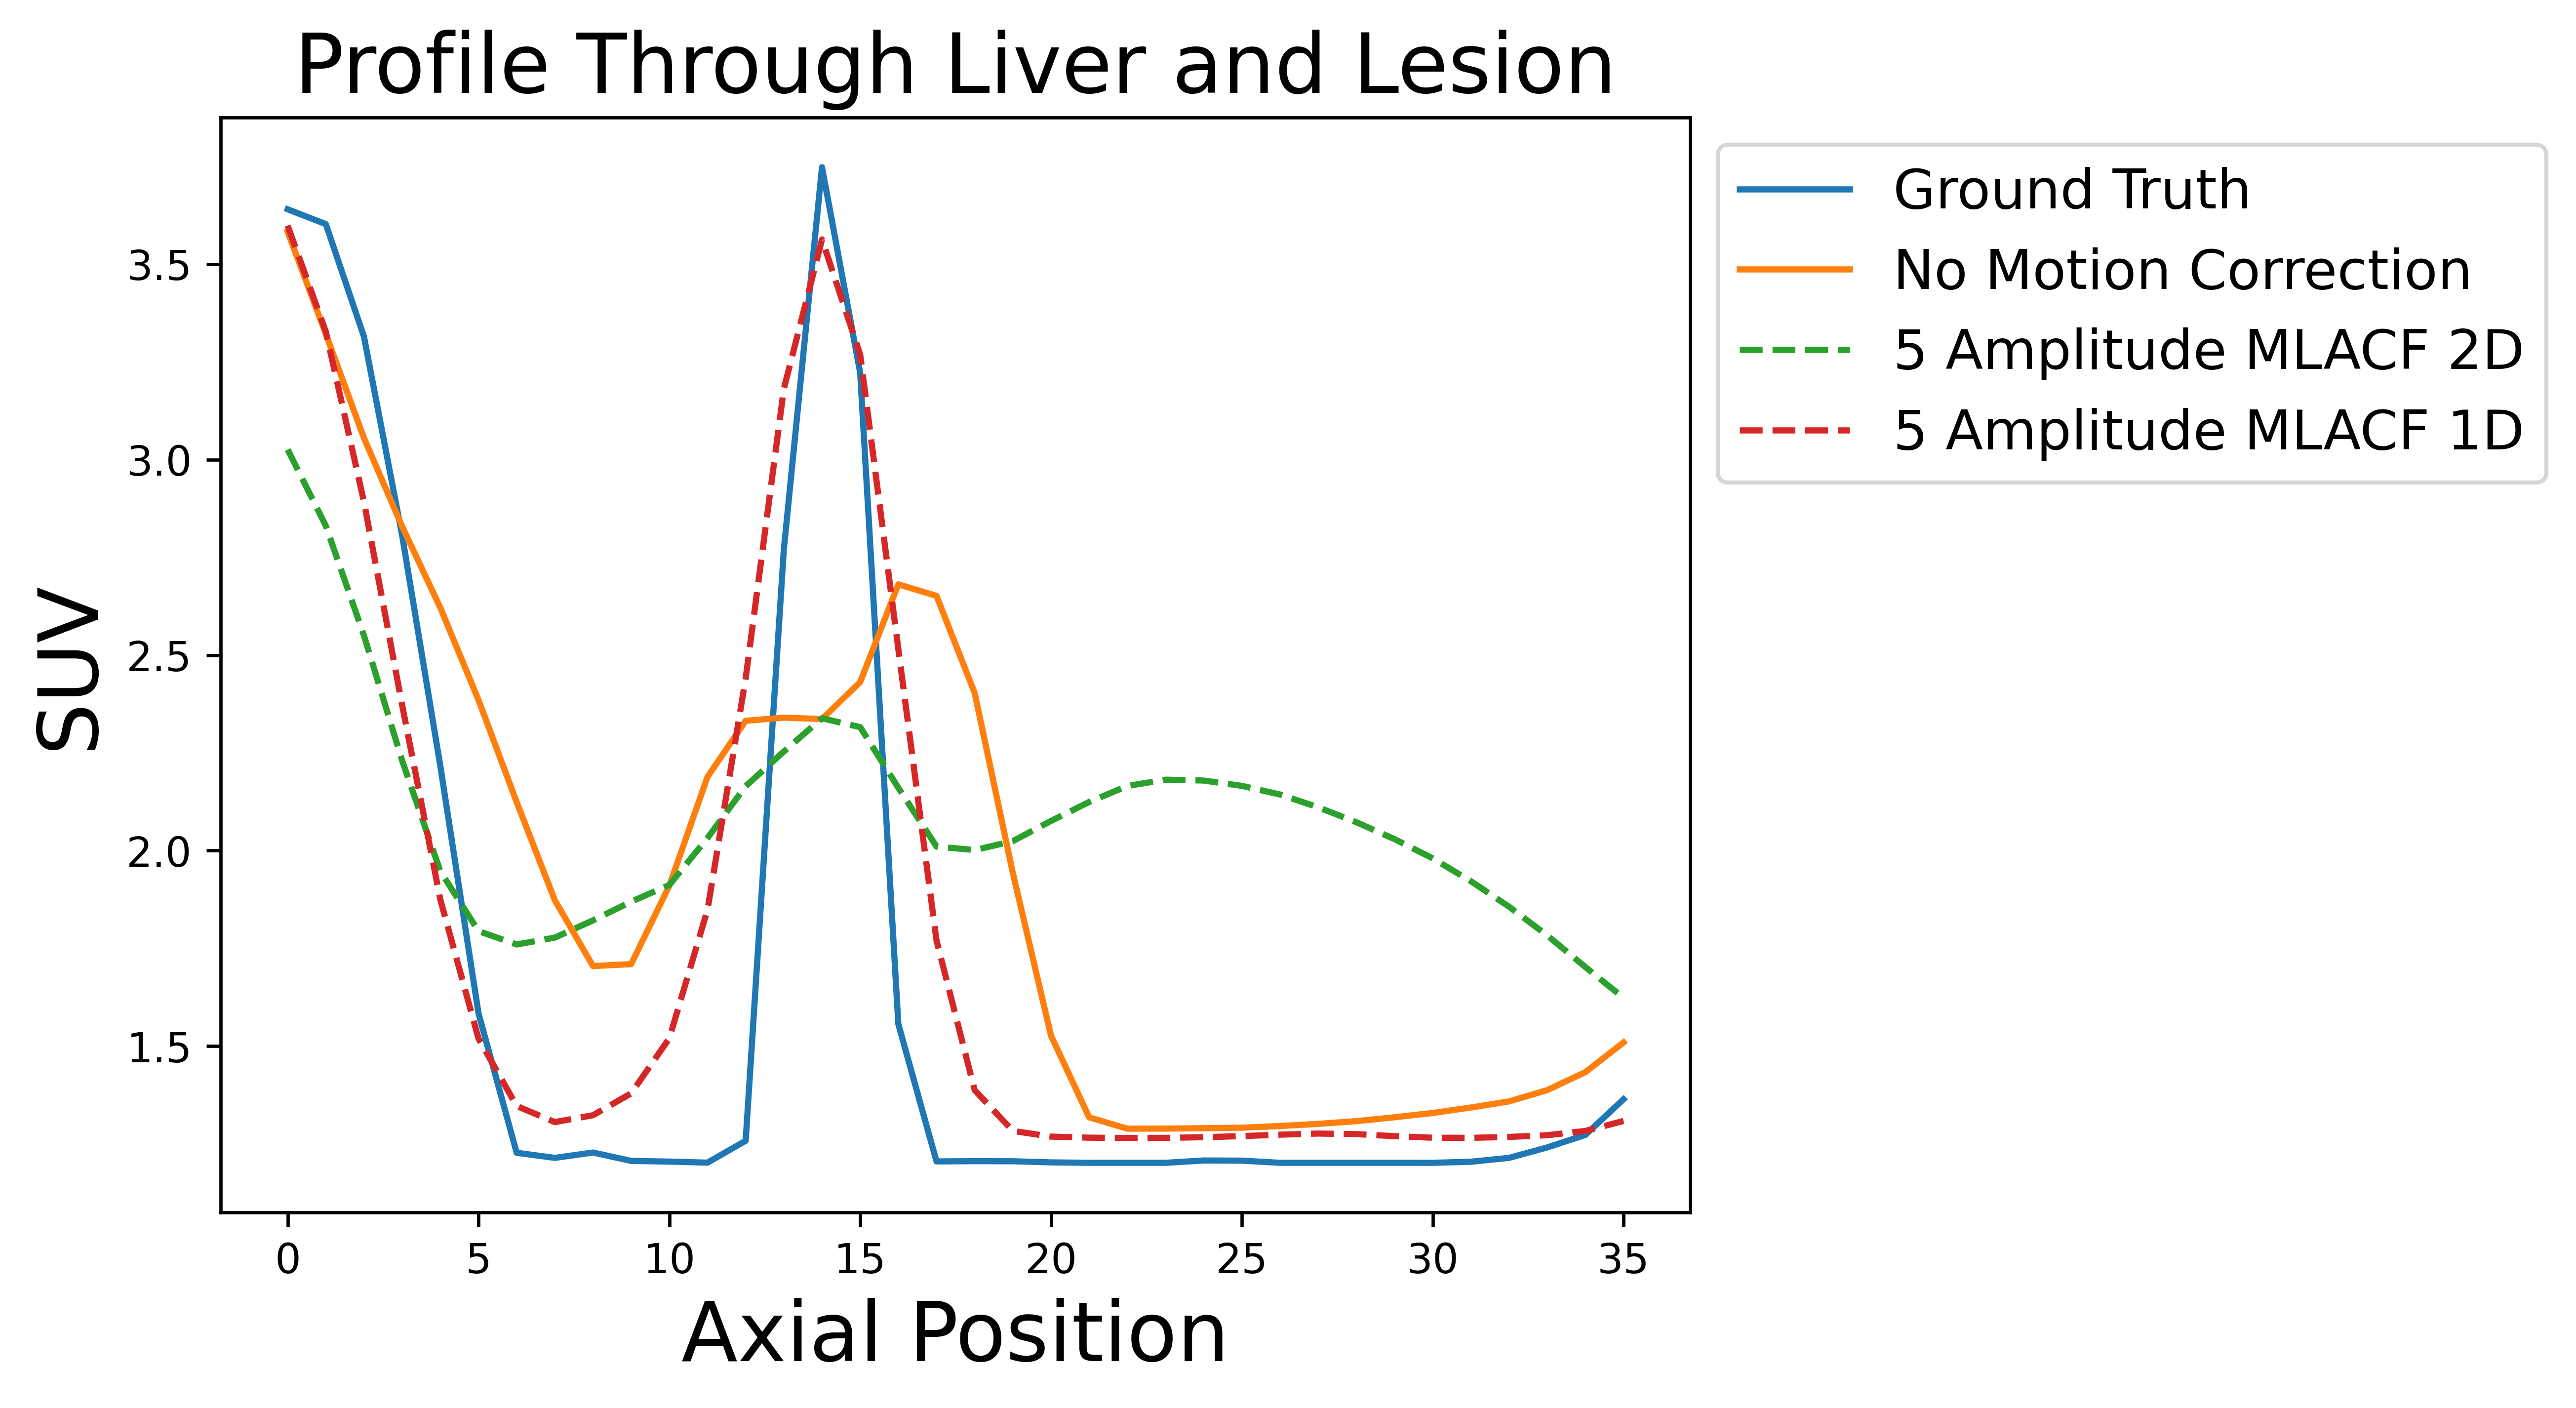
\includegraphics[width=1.0\linewidth]{figures/motion_correction_2_results_2_1d_vs_2d_profile.png}
                
                \captionsetup{singlelinecheck=false}
                \caption{
                    A profile through the lesion, in the \gls{SI} direction, summed over a window in the \gls{AP} and \gls{LM} directions, with median smoothing. This is for where different data was used to fit the \gls{MM} and the final \gls{MM} was applied to $30$ gate binned data. The data used to fit the \gls{MM} was as follows. Amplitude gated data with five bins reconstructed using \gls{MLACF}. Here, in the \gls{2D} case a \gls{2D} \gls{SS} was used and in the \gls{1D} case a \gls{1D} \gls{SS} was used. A \gls{MM} was also fit using a single bin, this is practically the equivalent of doing no motion correction.
                }
                
                \label{fig:evaluation_of_pet_ct_motion_correction_incorporating_motion_models_using_mlacf_and_complex_gating_schemes_results_1d_vs_2d_profile}
            \end{figure}

            \begin{figure}
                \centering
                
                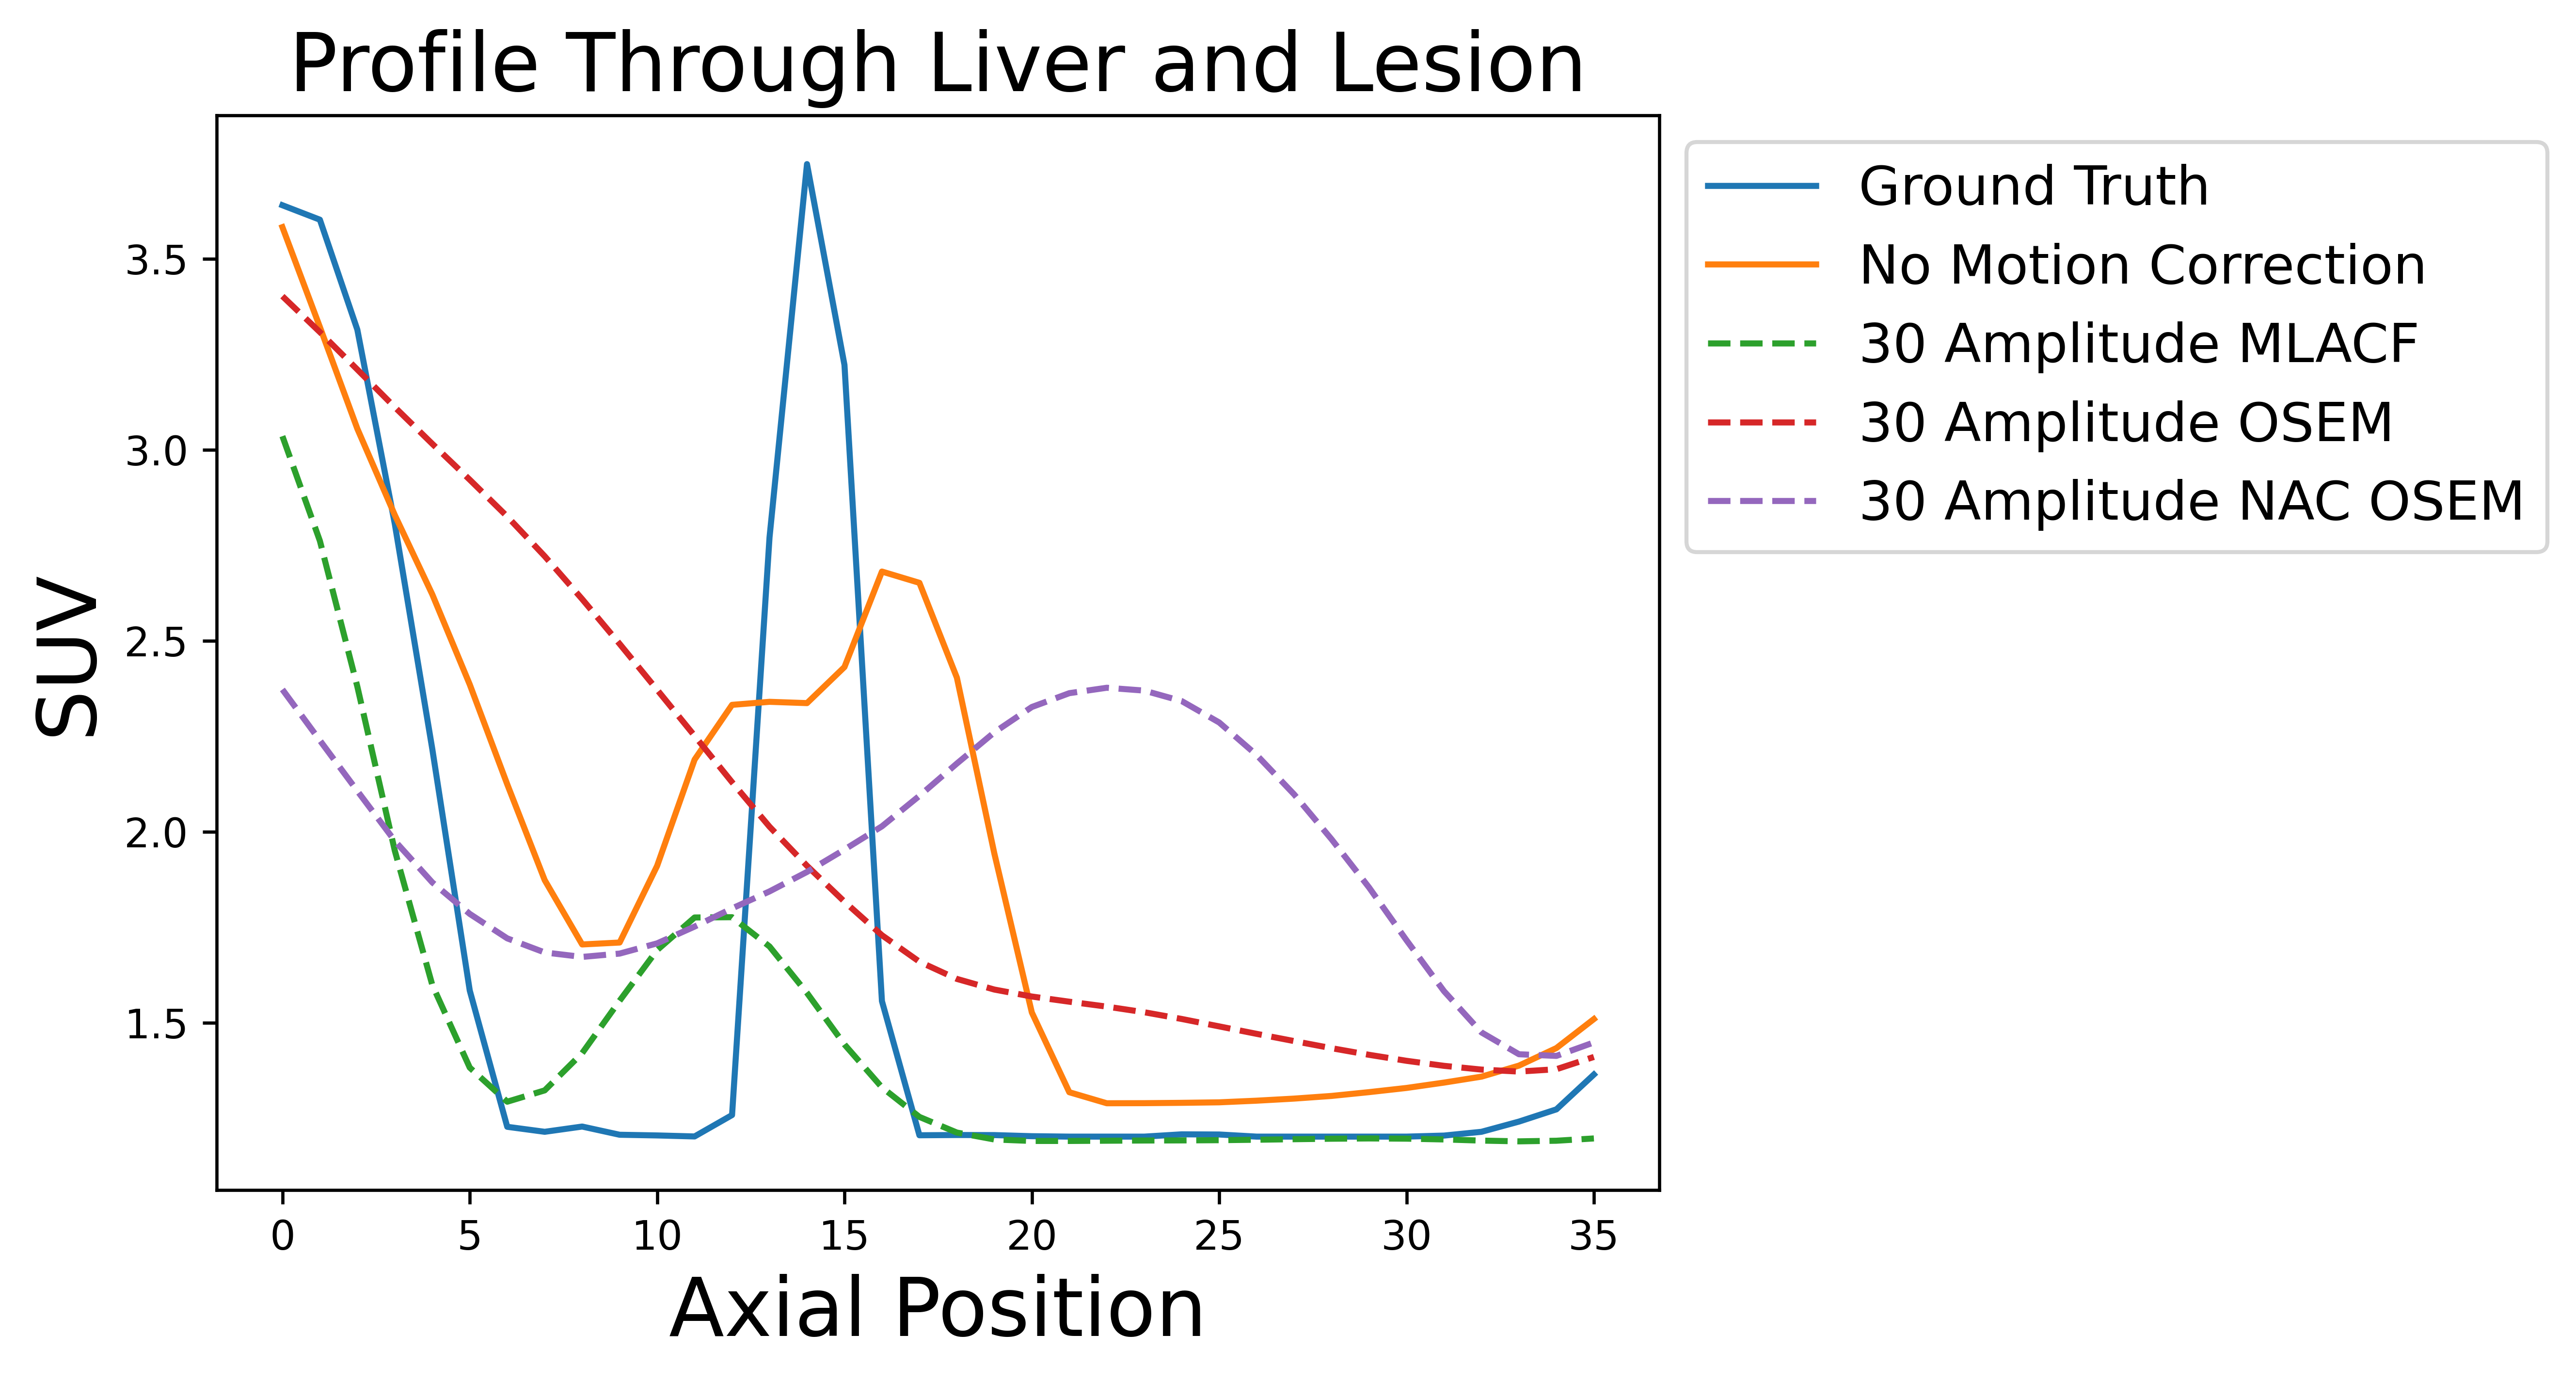
\includegraphics[width=1.0\linewidth]{figures/motion_correction_2_results_2_30_amplitude_profile.png}
                
                \captionsetup{singlelinecheck=false}
                \caption{
                    A profile through the lesion, in the \gls{SI} direction, summed over a window in the \gls{AP} and \gls{LM} directions, with median smoothing. This is where different data was used to fit the \gls{MM} and the final \gls{MM} was applied to $30$ gate binned data. The data used to fit the \gls{MM} was as follows. Amplitude gated data with $30$ bins reconstructed using \gls{MLACF}, \gls{AC} \gls{OSEM}, and \gls{NAC} \gls{OSEM}. A \gls{MM} was also fit using a single bin, which is practically the equivalent of doing no motion correction.
                }
                
                \label{fig:evaluation_of_pet_ct_motion_correction_incorporating_motion_models_using_mlacf_and_complex_gating_schemes_results_30_amplitude_profile}
            \end{figure}

            \begin{figure}
                \centering
                
                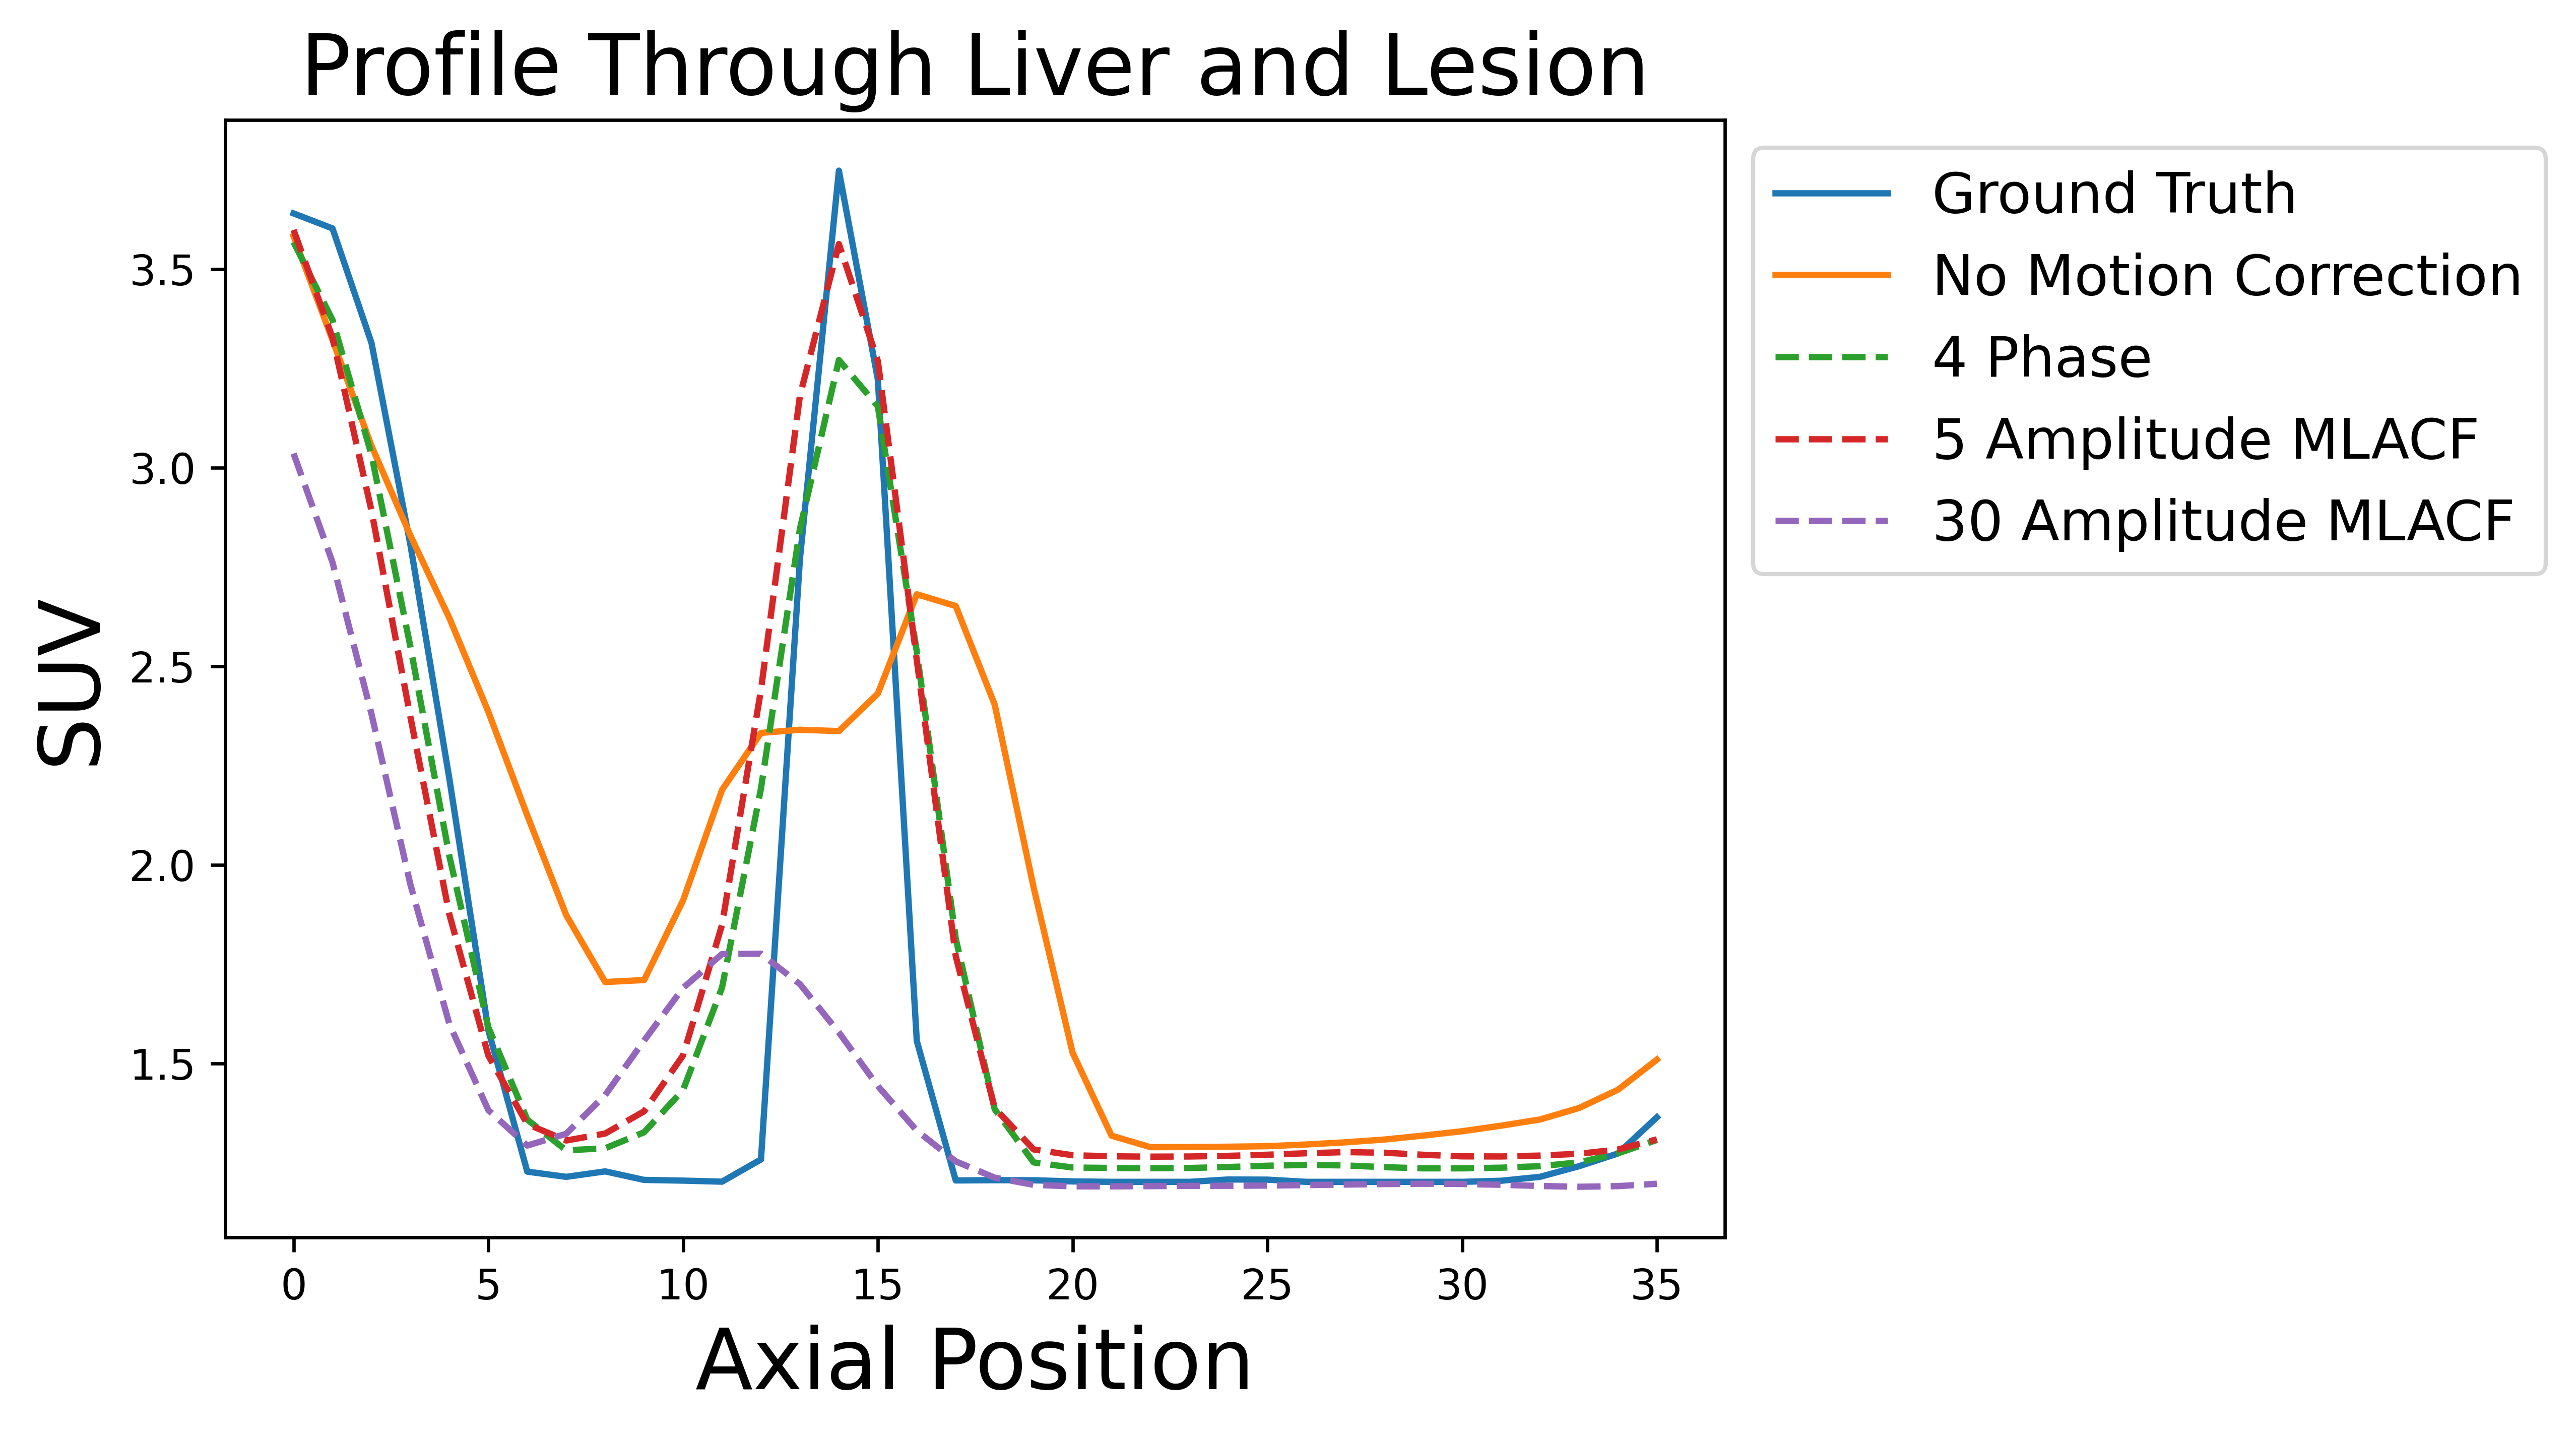
\includegraphics[width=1.0\linewidth]{figures/motion_correction_2_results_2_best_profile.png}
                
                \captionsetup{singlelinecheck=false}
                \caption{
                    A profile through the lesion, in the \gls{SI} direction, summed over a window in the \gls{AP} and \gls{LM} directions, with median smoothing. This is where different data was used to fit the \gls{MM} and the final \gls{MM} was applied to $30$ gate binned data. The methods presented here are a combination of the best one method from~\Fref{fig:evaluation_of_pet_ct_motion_correction_incorporating_motion_models_using_mlacf_and_complex_gating_schemes_results_phase_profile}, ~\Fref{fig:evaluation_of_pet_ct_motion_correction_incorporating_motion_models_using_mlacf_and_complex_gating_schemes_results_5_amplitude_profile}, and~\Fref{fig:evaluation_of_pet_ct_motion_correction_incorporating_motion_models_using_mlacf_and_complex_gating_schemes_results_30_amplitude_profile}. A \gls{MM} was also fit using a single bin, which is practically the equivalent of doing no motion correction.
                }
                
                \label{fig:evaluation_of_pet_ct_motion_correction_incorporating_motion_models_using_mlacf_and_complex_gating_schemes_results_best_profile}
            \end{figure}
            
            \begin{table}
                \centering
                
                \captionsetup{singlelinecheck=false}
                \caption{
                    Comparison of \gls{SUV}\textsubscript{max}, \gls{SUV}\textsubscript{median}, and \gls{SUV}\textsubscript{peak}, where different data was used to fit the \gls{MM} and the final \gls{MM} was applied to $30$ gate binned data. The data used to fit the \gls{MM} was as follows. `Phase' gated and \gls{MLACF} reconstructed data with three, four, eight and $12$ bins respectively. Amplitude gated data with five bins reconstructed using \gls{MLACF}, \gls{AC} \gls{OSEM}, and \gls{NAC} \gls{OSEM} (Here, in the \gls{2D} case a \gls{2D} \gls{SS} was used and in the \gls{1D} case a \gls{1D} \gls{SS} was used.). Amplitude gated data with $30$ bins reconstructed using \gls{MLACF}, \gls{AC} \gls{OSEM}, and \gls{NAC} \gls{OSEM}. A \gls{MM} was also fit using a single bin, which is practically the equivalent of doing no motion correction.
                }
                
                \resizebox*{1.0\linewidth}{!}
                {
                    \begin{tabular}{||c|ccc||}
                        \hline
                        \textbf{\gls{SUV}}                                      & \textbf{Max}  & \textbf{Median}   & \textbf{Peak} \\
                        \hline
                        \textbf{Ground Truth}                                   & $9.03$        & $2.47$            & $8.20$ \\
                        \textbf{No Motion Correction}                           & $5.69$        & $2.12$            & $4.31$ \\
                        \hline
                        \textbf{Three Phase}                                    & $8.09$        & $2.62$            & $5.78$ \\
                        \textbf{Four Phase}                                     & $7.48$        & $2.65$            & $5.75$ \\
                        \textbf{Eight Phase}                                    & $7.76$        & $1.42$            & $5.60$ \\
                        \textbf{12 Phase}                                       & $7.68$        & $1.30$            & $4.53$ \\
                        \hline
                        \textbf{Five Amplitude \gls{MLACF} \gls{2D}}            & $4.06$        & $1.75$            & $3.33$ \\
                        \textbf{Five Amplitude \gls{MLACF} \gls{1D}}            & $8.50$        & $2.31$            & $6.63$ \\
                        \textbf{Five Amplitude \gls{OSEM} \gls{1D}}             & $4.16$        & $1.40$            & $2.16$ \\
                        \textbf{Five Amplitude \gls{NAC} \gls{OSEM} \gls{1D}}   & $2.64$        & $1.34$            & $2.24$ \\
                        \hline
                        \textbf{30 Amplitude \gls{MLACF} \gls{1D}}              & $3.41$        & $1.21$            & $1.71$ \\
                        \textbf{30 Amplitude \gls{OSEM} \gls{1D}}               & $2.43$        & $1.38$            & $1.86$ \\
                        \textbf{30 Amplitude \gls{NAC} \gls{OSEM} \gls{1D}}     & $5.64$        & $1.28$            & $3.37$ \\
                        \hline
                    \end{tabular}
                }
                \label{tab:evaluation_of_pet_ct_motion_correction_incorporating_motion_models_using_mlacf_and_complex_gating_schemes_results_suv}
            \end{table}
            
            A visual analysis of the `phase' gated results with noise can be seen in~\Fref{fig:evaluation_of_pet_ct_motion_correction_incorporating_motion_models_using_mlacf_and_complex_gating_schemes_results_phase_visual_analysis} and without noise in~\Fref{fig:evaluation_of_pet_ct_motion_correction_incorporating_motion_models_using_mlacf_and_complex_gating_schemes_results_noiseless_phase_visual_analysis}. Here, it shows that the `phase' based gating approaches using \gls{MLACF} universally provide high quality results. The lesion appears more homogeneous and circular in all motion corrected results than in the non-motion corrected result. The Three Phase and Four Phase results are comparable and superior to the Eight Phase and Twelve Phase results. From what was observed in~\Fref{sec:pet_ct_motion_correction_exploiting_motion_models_fit_on_coarsely_gated_data_applied_to_finely_gated_data}, it is to be expected that with fewer gates comes a better performing motion correction method. However, the reduction in clarity of the lesion and diaphragm is obvious but less than might be expected when compared to where $30$ gates are used in~\Fref{sec:pet_ct_motion_correction_exploiting_motion_models_fit_on_coarsely_gated_data_applied_to_finely_gated_data_results}. The \gls{PIQE} results support this, the values for the Three Phase and Four Phase methods are greater than the Eight Phase and Twelve Phase methods. The \gls{PIQE} values for the Three Phase and Four Phase are also greater than where no motion correction is used and are closest to the ground truth \gls{PIQE} values.
            
            A visual analysis of the amplitude gated results using five bins with noise are shown in~\Fref{fig:evaluation_of_pet_ct_motion_correction_incorporating_motion_models_using_mlacf_and_complex_gating_schemes_results_5_amplitude_visual_analysis} and without noise in~\Fref{fig:evaluation_of_pet_ct_motion_correction_incorporating_motion_models_using_mlacf_and_complex_gating_schemes_results_noiseless_5_amplitude_visual_analysis}. Here, it can be seen that \gls{MLACF} (when used with amplitude gating of five bins) significantly improves results when compared to \gls{AC} and \gls{NAC} \gls{OSEM}. The lesion in the \gls{MLACF} example is comparable to the lesions present in the `phase' based results. However, for both the \gls{AC} and \gls{NAC} \gls{OSEM} results the lesion does not appear in the same location as in the ground truth and also looks very non-homogeneous. The results from both \gls{OSEM} methods actually seem to be worse than doing no motion correction at all. The \gls{PIQE} values somewhat support this, however \gls{PIQE} appears to have erroneously scored the \gls{NAC} \gls{OSEM} results highly. This erroneous scoring could be attributed to this image being smoother and thus potentially more perceptually pleasing.
            
            A visual analysis of the difference between the amplitude gated results with five bins using a \gls{2D} and a \gls{1D} \gls{SS} with noise can be seen in~\Fref{fig:evaluation_of_pet_ct_motion_correction_incorporating_motion_models_using_mlacf_and_complex_gating_schemes_results_1d_vs_2d_visual_analysis} and without noise in~\Fref{fig:evaluation_of_pet_ct_motion_correction_incorporating_motion_models_using_mlacf_and_complex_gating_schemes_results_noiseless_1d_vs_2d_visual_analysis}. Here, it could be hypothesised that a \gls{2D} \gls{SS} is detrimental to motion correction when compared to a \gls{1D} \gls{SS}. However, it is more likely that the results for the \gls{2D} \gls{SS} are caused by a lack of constraint along the gradient dimension. A \gls{2D} \gls{SS} is used for all `phase' based methods, which show good results. The \gls{PIQE} results support this, the values for the \gls{2D} \gls{SS} are very low.
            
            A visual analysis of the amplitude gated results using $30$ bins with noise can be seen in~\Fref{fig:evaluation_of_pet_ct_motion_correction_incorporating_motion_models_using_mlacf_and_complex_gating_schemes_results_30_amplitude_visual_analysis} and without noise in~\Fref{fig:evaluation_of_pet_ct_motion_correction_incorporating_motion_models_using_mlacf_and_complex_gating_schemes_results_noiseless_30_amplitude_visual_analysis}. Here, it shows that all methods which utilised $30$ bins have failed. This supports the results shown in~\Fref{sec:pet_ct_motion_correction_exploiting_motion_models_fit_on_coarsely_gated_data_applied_to_finely_gated_data}. As with the \gls{PIQE} values for the five bin methods, the \gls{PIQE} values here are suspiciously high. This again could potentially be caused by the smoothness of the images where motion correction has failed.
            
            A visual analysis of the best results from the previous analysis with noise can be seen in~\Fref{fig:evaluation_of_pet_ct_motion_correction_incorporating_motion_models_using_mlacf_and_complex_gating_schemes_results_best_visual_analysis} and without noise in~\Fref{fig:evaluation_of_pet_ct_motion_correction_incorporating_motion_models_using_mlacf_and_complex_gating_schemes_results_noiseless_best_visual_analysis}. In this case, the Four Phase and Five Amplitude methods perform relatively comparably (and significantly better than the Thirty Amplitude results where motion correction has failed). The lesion and diaphragm in the Four Phase and Five Amplitude cases both show a significant improvement over where no motion correction is used. The Four Phase and Five Amplitude methods both contain a lesion in the same location, and of a similar shape, when compared to the ground truth. The results potentially lead to the conclusion that, with the data used here, it is more important to use fewer bins when gating than it is to use a \gls{2D} \gls{SS}. \gls{PIQE} values appear potentially inconclusive when the values from the Thirty Amplitude method are taken into account.

            A profile across the lesion for the `phase' gated results is presented in~\Fref{fig:evaluation_of_pet_ct_motion_correction_incorporating_motion_models_using_mlacf_and_complex_gating_schemes_results_phase_profile}. Here, again it can be seen that the Three Phase and Four Phase methods provide profiles with the highest peaks and which most closely match the ground truth. When compared to the visual analysis, it is more obvious that there is a degradation in quality as the number of bins used increases. The Twelve Phase method has a much lower peak which is shifted to the left.
            
            A profile across the lesion for the amplitude gated results using five bins is shown in~\Fref{fig:evaluation_of_pet_ct_motion_correction_incorporating_motion_models_using_mlacf_and_complex_gating_schemes_results_5_amplitude_profile}. Here, it can be seen that the \gls{MLACF} based method provides an exceptionally good profile. More specifically, the \gls{MLACF} based method has a profile where the peak almost exactly matches the ground truth. However, the width of the peak for the \gls{MLACF} method is much greater than the ground truth. The other methods shown here appear to have completely failed, their peak is heavily shifted to the right and is much lower than the \gls{MLACF} based method.
            
            A profile across the lesion showing the difference between the amplitude gated results with five bins using a \gls{2D} and a \gls{1D} \gls{SS} can be seen in~\Fref{fig:evaluation_of_pet_ct_motion_correction_incorporating_motion_models_using_mlacf_and_complex_gating_schemes_results_1d_vs_2d_profile}. Here, it shows that the \gls{2D} \gls{SS} method has failed. Although the peak of the \gls{2D} \gls{SS} method is in the same place as in the ground truth, there is an additional erroneous peak to its right.
            
            A profile across the lesion for the amplitude gated results using $30$ bins is presented in~\Fref{fig:evaluation_of_pet_ct_motion_correction_incorporating_motion_models_using_mlacf_and_complex_gating_schemes_results_30_amplitude_profile}. Here, it can be seen that all methods utilising a large number of bins have failed entirely. If there is a peak in the profile, then it does not match the scale or location of the ground truth at all.
            
            A profile across the lesion showing best results from the previous profiles can be seen in~\Fref{fig:evaluation_of_pet_ct_motion_correction_incorporating_motion_models_using_mlacf_and_complex_gating_schemes_results_best_profile}. This shows that the Four Phase and Five Amplitude methods provide very similar profiles. Although the peak of the Five Amplitude method may be greater than the peak of the Four Phase method, it is also true that the width of the peak for the Four Phase method is less than that of the Five Amplitude method. Additionally, the Four Phase method very slightly matches the ground truth more closely outside the peak, for instance, where the diaphragm is.

            \gls{SUV}\textsubscript{max}, \gls{SUV}\textsubscript{median}, and \gls{SUV}\textsubscript{peak} results can be seen for all methods in~\Fref{tab:evaluation_of_pet_ct_motion_correction_incorporating_motion_models_using_mlacf_and_complex_gating_schemes_results_suv}. An analysis of \gls{SUV} results shows the following.

            \begin{itemize}
                \item For \gls{SUV}\textsubscript{max} results, the Three Phase and Five Amplitude (using \gls{MLACF}) methods have values which most closely match the ground truth when compared to other methods. All Thirty Gate and \gls{OSEM} methods have a very low \gls{SUV}\textsubscript{max} value. Strangely, the Four Phase method has a lower \gls{SUV}\textsubscript{max} than the Eight Phase and Twelve Phase methods. This could be attributed to the fact that \gls{SUV}\textsubscript{max} is very susceptible to noise.

                \item For \gls{SUV}\textsubscript{median} results, the Three Phase and Four Phase methods have exceptionally high values. These values are even higher than the ground truth, potentially leading to the conclusion that the `phase' based methods have shrunk the size of the lesion when compared to the ground truth. The Five Amplitude method (using \gls{MLACF}) has a lower \gls{SUV}\textsubscript{median} but one which is close to the ground truth.

                \item For \gls{SUV}\textsubscript{peak} results, the Five Amplitude (using \gls{MLACF}) method has a very good score which is closest to the ground truth. The Three Phase and Four Phase methods have values which are very close to each other but they lag behind the Five amplitude (using \gls{MLACF}) method.
            \end{itemize}

        \subsection{Conclusion} \label{sec:evaluation_of_pet_ct_motion_correction_incorporating_motion_models_using_mlacf_and_complex_gating_schemes_conclusion}
            In conclusion, after a thorough analysis of the results visually, both of their profile through the lesion as well as of their \gls{SUV}, it can be shown that the Four Phase and Five Amplitude (using \gls{MLACF}) methods most often provide the best results. The Four Phase method had a narrower peak in the profile (closer to the ground truth) and more closely matched values outside of the lesion. However, the Five Amplitude (using \gls{MLACF}) method had a greater peak in the profile (closer to the ground truth) and more often had superior \gls{SUV}. Although this is the case, it should be noted that both methods significantly outperformed other methods. For instance, all \gls{OSEM} and all methods with a large number of bins unanimously failed.
            
            When compared to the methods which failed, it is more interesting to highlight what the two best methods share in common, rather than what separates them. The two best methods both used \gls{MLACF} and a small number of bins. It appears from experiments here, but also when comparing~\Fref{sec:subsequent_motion_correction_using_advanced_reconstruction_and_gating_methods_with_more_challenging_data} and~\Fref{sec:initial_motion_correction_using_basic_reconstruction_and_gating_methods_with_less_challenging_data}, that when low count data is used, \gls{MLACF} is almost a necessity for accurate motion correction. Furthermore, the fact that a low number of bins is beneficial when applying motion correction shows a benefit for \glspl{MM}. This is because using a low number of bins for motion correction but then applying this motion correction to a high number of bins would not be possible without motion modelling.
            
            However, when it comes to the benefits of \gls{2D} gating, it could be argued that results here are inconclusive. This is potentially due to the fact that rationally modelling hysteresis is more beneficial than not modelling it. It could be argued that the simulated data used here was not complex enough to show this.
        
    \section{Discussion} \label{sec:subsequent_motion_correction_using_advanced_reconstruction_and_gating_methods_with_more_challenging_data_discussion}
        The discussion presented here will be with respect to the discussion in~\Fref{sec:initial_motion_correction_using_basic_reconstruction_and_gating_methods_with_less_challenging_data_discussion}. The discussion will highlight where progress has been made when compared to the issues and limitations raised previously. Here, potential future directions will also be discussed to further the aims of rectifying these problems.

        Firstly, the most obvious flaw with the work presented here is that it has still not been evaluated using patient data. The work performed for~\Fref{sec:evaluation_of_pet_ct_motion_correction_incorporating_motion_models_using_mlacf_and_complex_gating_schemes} was intended to get the implementation ready to use patient data. However, as it always is, things are often more difficult than they originally appear. Many issues with the method were found when it began to be applied to patient data. Most of these issues were related to the swap from \gls{2D} to \gls{3D} acquisition simulations and the decrease in the \gls{TOF} resolution. Furthermore, the reconstruction method had never been tested before with randoms, scatter, and a normalisation sinogram input. The reconstruction method was already not robust when used in~\Fref{sec:pet_ct_motion_correction_exploiting_motion_models_fit_on_coarsely_gated_data_applied_to_finely_gated_data} and failed entirely when the simulation data was made more realistic. The changes made in~\Fref{sec:evaluation_of_pet_ct_motion_correction_incorporating_motion_models_using_mlacf_and_complex_gating_schemes} allowed the method to be used end to end with real \gls{GE} Discovery $710$ patient data (the method was tested with a single gate as input and produced reasonable non-motion corrected results). The one thing preventing the method from being tested with patient data is a way to split the acquired patient data into \SI{0.5}{\hertz} sinograms. This is actually quite a trivial change, however, the problem lies in the assumption made that many \SI{0.5}{\hertz} sinograms is a sensible input. The number of sinograms required for the patient data, especially if it is a dynamic acquisition, uses a significant amount of storage. If this is to be changed in the implementation itself, then a not insignificant amount of work would be required. Regardless, although patient data results may not be available at the time of writing, a paper is in the process of being written, which will incorporate the patient data results, when they are ready.

        As began to be addressed in~\Fref{sec:comparison_of_motion_correction_methods_incorporating_motion_modelling_for_pet_ct_using_a_single_breath_hold_attenuation_map}, the \gls{XCAT} simulations used in this chapter uniformly use \glspl{SS} derived from \gls{CMR} to drive the respiratory model. This addresses the limitation mentioned previously where there was no breath to breath variability present in the data. This was due to only one \gls{SS} being used which is repeated for each breath.

        The anatomy used for the \gls{XCAT} simulations still did not vary (it was the average male anatomy). However, as began to be addressed in~\Fref{sec:comparison_of_motion_correction_methods_incorporating_motion_modelling_for_pet_ct_using_a_single_breath_hold_attenuation_map} and as is mentioned in~\Fref{sec:pet_ct_motion_correction_exploiting_motion_models_fit_on_coarsely_gated_data_applied_to_finely_gated_data_methods_xcat_volume_generation}, the lesion was made much smaller and moved much closer to the diaphragm. The lesion was small enough that from the minimum displacement to the maximum displacement, due to respiration, the lesion would not overlap with itself. Furthermore, the lesion was placed close enough to the diaphragm that from the minimum displacement to the maximum displacement, due to respiration, the lesion is fully within the area where the diaphragm was at the opposite respiratory state.

        As was discussed in~\Fref{sec:evaluation_of_pet_ct_motion_correction_incorporating_motion_models_using_mlacf_and_complex_gating_schemes_methods_xcat_volume_generation_and_pet_acquisition_simulation}, the method to simulate the \gls{PET} acquisition is now significantly more realistic. A relatively low count rate is used, at the level of a research scan count rate. A pseudo-random and scatter simulation was used to emulate the randoms and scatter profile seen in patient data. This is not a true random and scatter simulation, due to software limitations when using \gls{TOF}. However, care was taken to make the simulations as realistic as possible given the constraints.

        Again, as was discussed in~\Fref{sec:evaluation_of_pet_ct_motion_correction_incorporating_motion_models_using_mlacf_and_complex_gating_schemes_methods_xcat_volume_generation_and_pet_acquisition_simulation}, the \gls{TOF} resolution for the \gls{PET} acquisition simulation was reduced to that of the \gls{GE} Discovery $710$. This did have a noticeable effect on the quality of the reconstructed and motion corrected volumes. However, the method was improved so that similar performance was seen as before the resolution was reduced.

        The registrations used universally in this chapter employed \gls{NMI} as an objective function. This even included in~\Fref{sec:evaluation_of_pet_ct_motion_correction_incorporating_motion_models_using_mlacf_and_complex_gating_schemes_methods_registration_motion_model_estimation_and_motion_corrected_image_reconstruction_with_attenuation_correction} where the reference volume was selected for pair-wise registration. \gls{NMI} appears to be universally superior to \gls{SSD} or \gls{MSE}, especially when performing registration between two modalities (like \gls{PET} and \gls{CT}). If \gls{NMI} is used for all registrations, including where the same modality is used, it makes the hyperparameter tuning easier due to the parameters being similar for both types of registration. Furthermore, although the work in this chapter continued to fit the registration and \gls{MM} separately, it never appeared to be the limiting factor for the quality of the motion correction. It would be interesting to compare two motion correction algorithms where the only differentiating factor is how the \gls{MM} is fit. However, such a comparison seems difficult due to how differently both methods would need to be implemented.
        
        The \glspl{MM} used in this chapter continued to be fit as a linear regression, this could be considered to be a limitation of the method. However, it could also be the case that especially where few bins are used (as was found to be beneficial by the work in this chapter) that it would not be possible to benefit from a more complex type of model. If a more complex model was used here (for instance a type of non-linear regression), it is more likely that it would begin to overfit and not offer any kind of regularisation of the \gls{DVF} results.

        For the sinogram space objective function critique, a conscious effort to maximise the potential of image space based objective functions was made. Although it is true that sinogram space objective function could provide the benefits listed in~\Fref{sec:initial_motion_correction_using_basic_reconstruction_and_gating_methods_with_less_challenging_data_discussion}, it is also true that these methods add significant implementation complexity and increased execution time. The results presented in this chapter appear satisfactory. If a sinogram space objective function is unnecessary, then the method would have the benefit of simplified implementation and reduced execution time. For clinical adoption the shortest execution time is often beneficial.

        Any points not otherwise mentioned above from~\Fref{sec:initial_motion_correction_using_basic_reconstruction_and_gating_methods_with_less_challenging_data_discussion} have not been addressed and the same issues still stand.
